\documentclass{report}

\usepackage{float}
\usepackage{titlesec}
\usepackage{graphicx}
\usepackage{amsmath}
\usepackage{subcaption}
\usepackage{listings}
\usepackage{xcolor}
\usepackage{apacite}
\usepackage{url}
\usepackage{tikz}

\bibliographystyle{apacite}

\graphicspath{ {./assets/} {..} }

\newcommand{\subimgw}{.7\linewidth}

\definecolor{codegreen}{rgb}{0,0.6,0}
\definecolor{codegray}{rgb}{0.5,0.5,0.5}
\definecolor{codepurple}{rgb}{0.58,0,0.82}
\definecolor{backcolour}{rgb}{0.95,0.95,0.92}

\lstdefinestyle{mys}{
    backgroundcolor=\color{backcolour},   
    commentstyle=\color{codegreen},
    keywordstyle=\color{magenta},
    numberstyle=\tiny\color{codegray},
    stringstyle=\color{codepurple},
    basicstyle=\ttfamily\footnotesize,
    breakatwhitespace=false,
    breaklines=true,
    captionpos=b,
    keepspaces=true,
    numbers=left,
    numbersep=5px,
    showspaces=false,
    showstringspaces=false,
    showtabs=false,
    tabsize=2
}
\lstset{style=mys}

\author{
  Kristian Henrik Salen Sørli
  \and
  William B. Sørensen\\
}
\title{TOF Rapport}
\begin{document}
\maketitle

\tableofcontents

\chapter{Glossary}

\begin{figure}[H]
	\centering
	\begin{tabular}{|c|c|}
		\hline
		Term       & Definition                                       \\
		\hline
		Arch       & The loadbering arch of the bridge; overgurt      \\
		Baselines  & The main base for the bridge; undergurt          \\
		Nodes      & The structural nodes of the model                \\
		Beams      & The wooden beams between the nodes               \\
		Rods       & The PLA shroud around the beams                  \\
		SCAD space & Nodes with the indexing scheme used in Open SCAD \\
		JHU space  & Nodes with the indexing scheme used in JHU       \\
		\hline
	\end{tabular}
	\caption{Glossary}
\end{figure}

\chapter{Tasks}

% Task 1: Utforske styrken til geometriske strukturer

% 1A: Lag formene nedenfor ved å bruke spagetti og limpistol. Undersøk og sammenlign strukturene sin evne til å bære en vertikal last. Undersøk og sammenlign også hvordan formene reagerer på horisontal last.

% I besvarelsen må dere ta med figurenes korrekte navn, skisse av strukturene og spagetti-strukturene, resultatene fra testingen, teori som kan forklare resultatene dere får fra testingen og endelig konklusjon.

% 1B: Lag formene nedenfor ved å bruke spagetti og limpistol. Undersøk og sammenlign strukturene sin evne til å bære en vertikal last. Undersøk og sammenlign også hvordan formene reagerer på horisontal last.

% I besvarelsen må dere ta med figurenes korrekte navn, skisse av strukturene og spagetti-strukturene, resultatene fra testingen, teori som kan forklare resultatene dere får fra testingen og endelig konklusjon.

\section{Task 1}

\subsection{A}

In this task we designed an array of polygons out of spaghetti. This was to see and order the strength of the different polygons.

From a polygonal perspective the most uniformly integral entity was the equilateral triangle. This stems from its ability to support an equal amount of force (both contraction and compression) from each plane of translation. You can see our representation as Figure \ref{fig:eq}.

\begin{figure}[H]
	\centering
	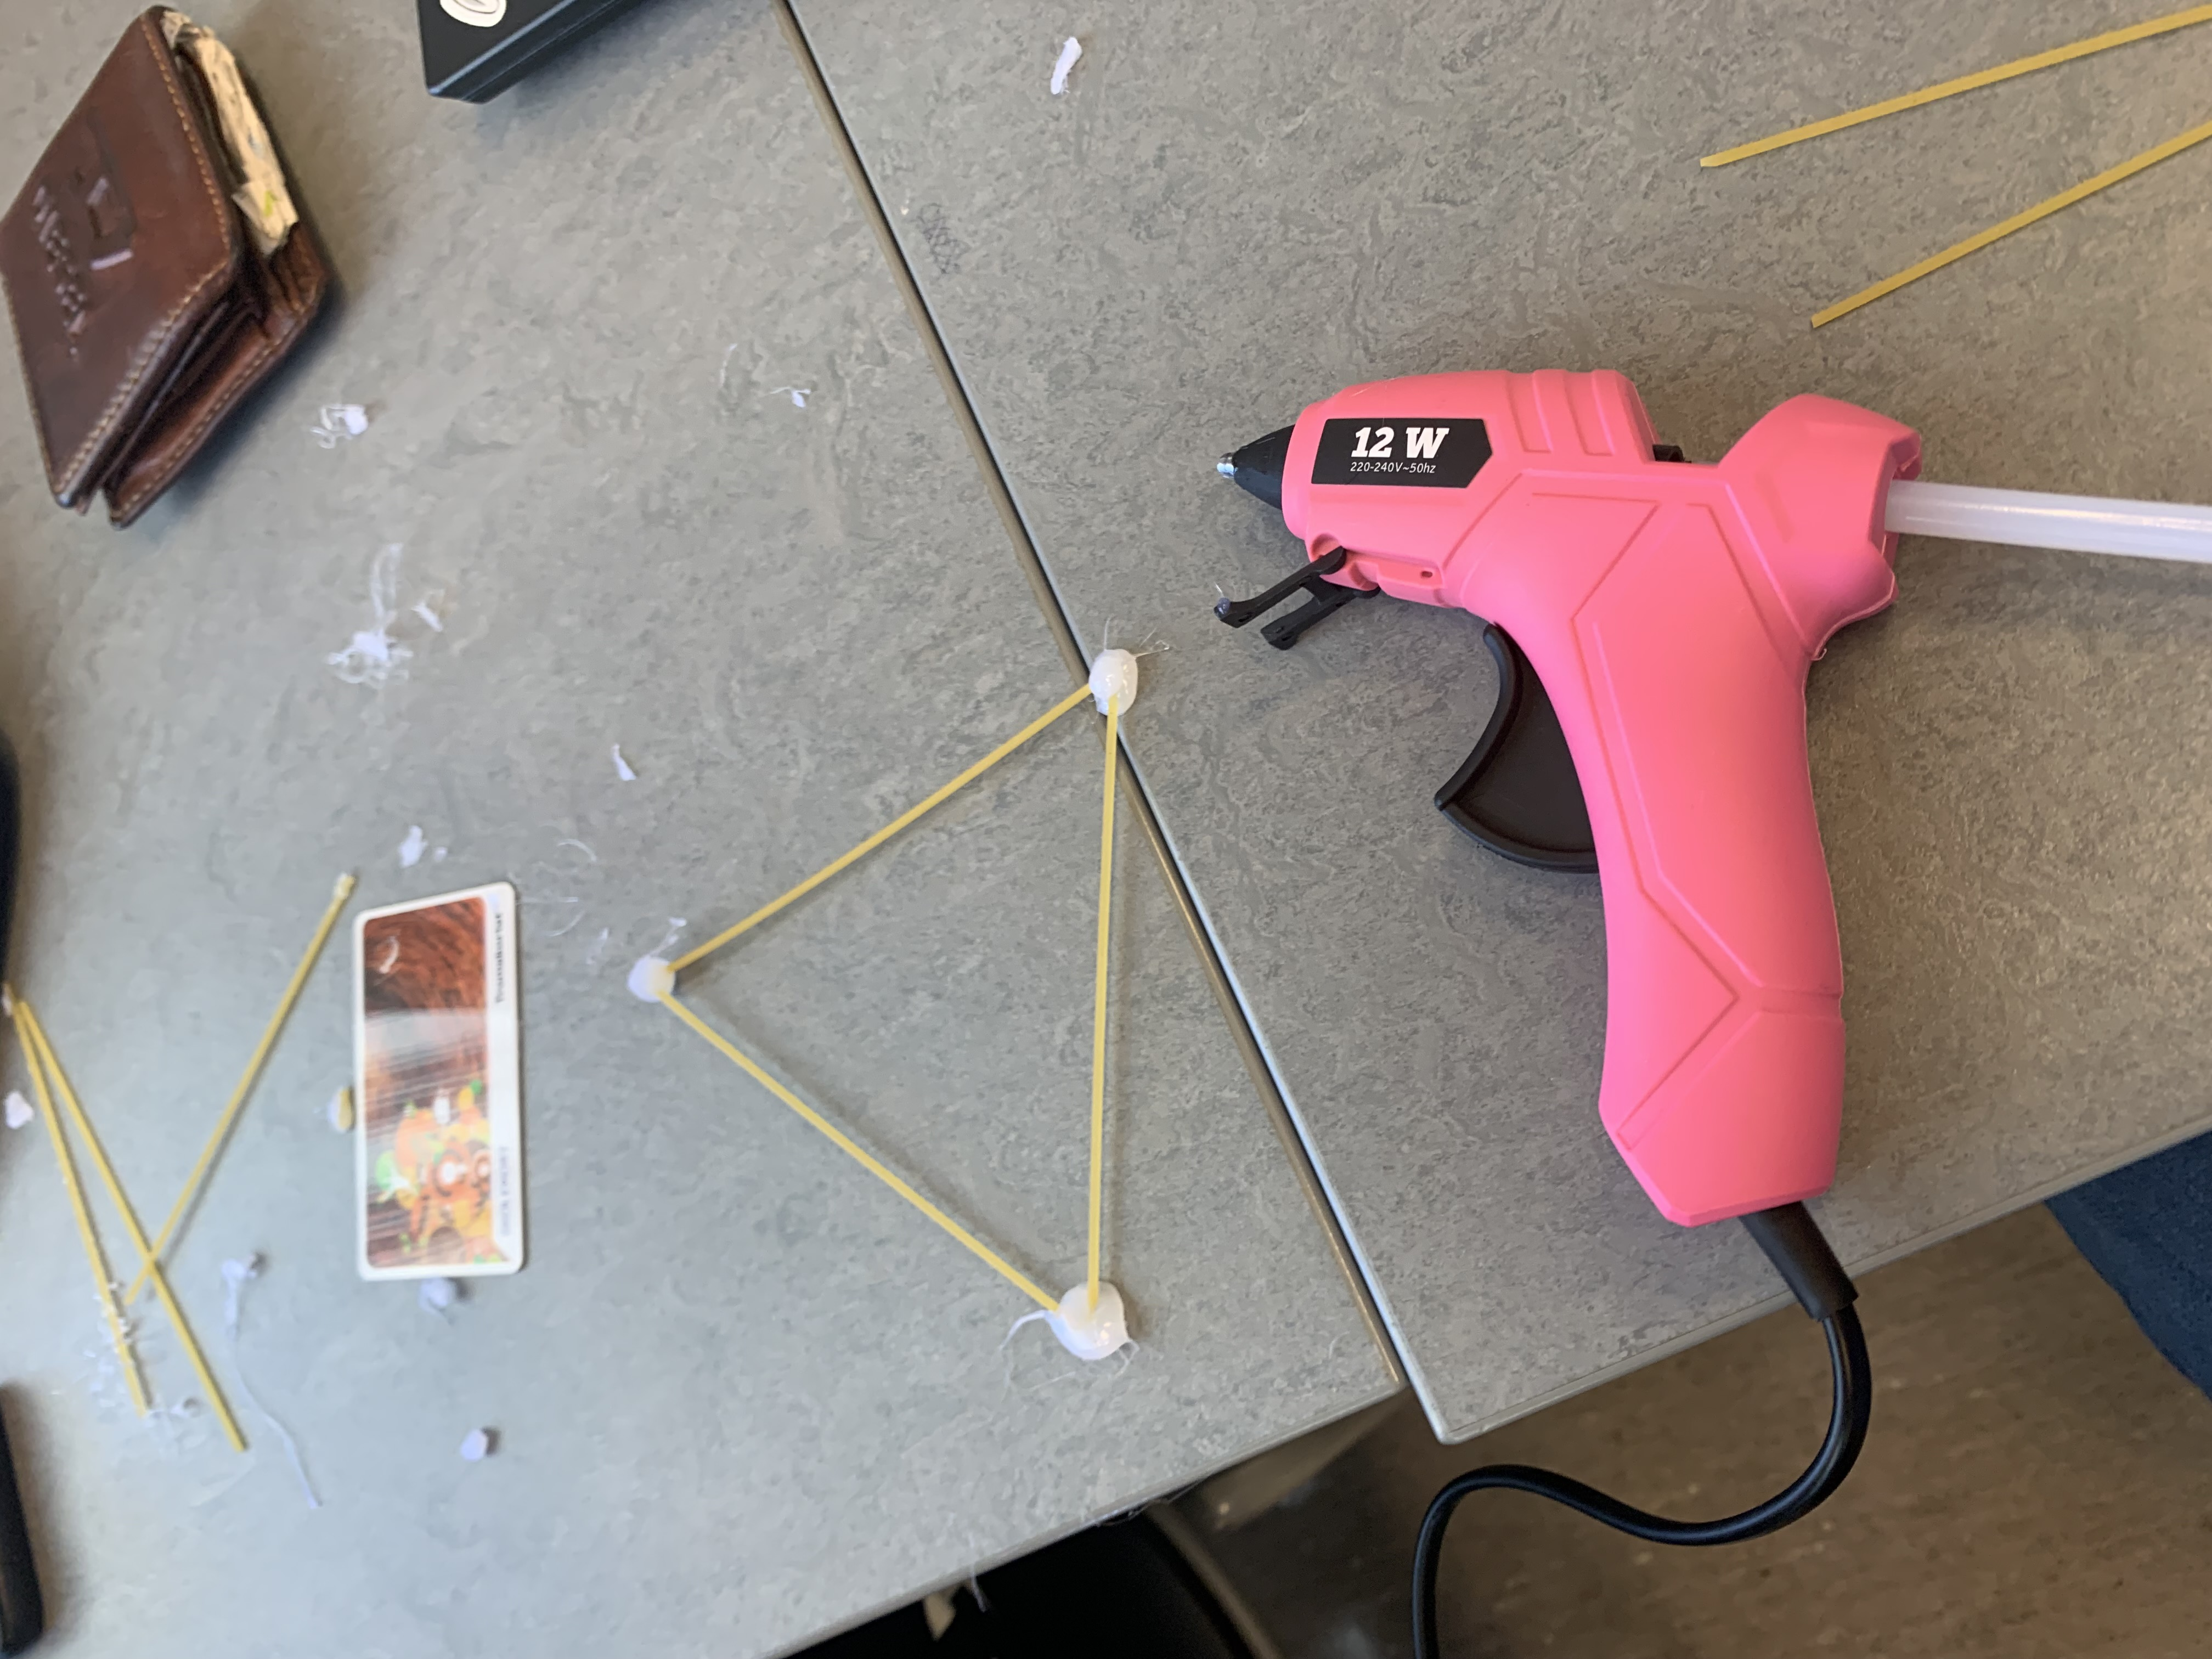
\includegraphics[width=.8\linewidth]{equalateral}

	\caption {Equilateral triangle}
	\label{fig:eq}
\end{figure}

An isosceles triangle follows suit from the equilateral triangle through the fact that its similarity to this shape dictates how uniformly it displaces its forces. We can inspect greater buckling along the major axiis something that can be explained by the added length. This results in the polygon being weakest to compression-forces along its longest sides

A square is the weakest possible shape as it falls pray to plane translation as it is implicitly a compliant mechanism.

This results in a strength ordering of:

\begin{enumerate}
	\item Equilateral triangle
	\item Isosceles triangle
	\item Square
\end{enumerate}

\subsection{B}

A tetrahedron has the same strengths as an equilateral triangle originating from the fact that its comprised of 4 (tetra) equilateral triangles. This means it equally balances forces through each beam. This is highly useful for a truss perspective and can be observed in trusses in other situations but for a bridge construction it is simply not practical. An example of this is the ISS of which trusses like this are used for the solar array \cite{wiki:itruss}. See Figure \ref{fig:itruss} for image. One can see an example of a tetrahedron we designed in Figure \ref{fig:tetrehedra}.

\begin{figure}[H]
	\centering
	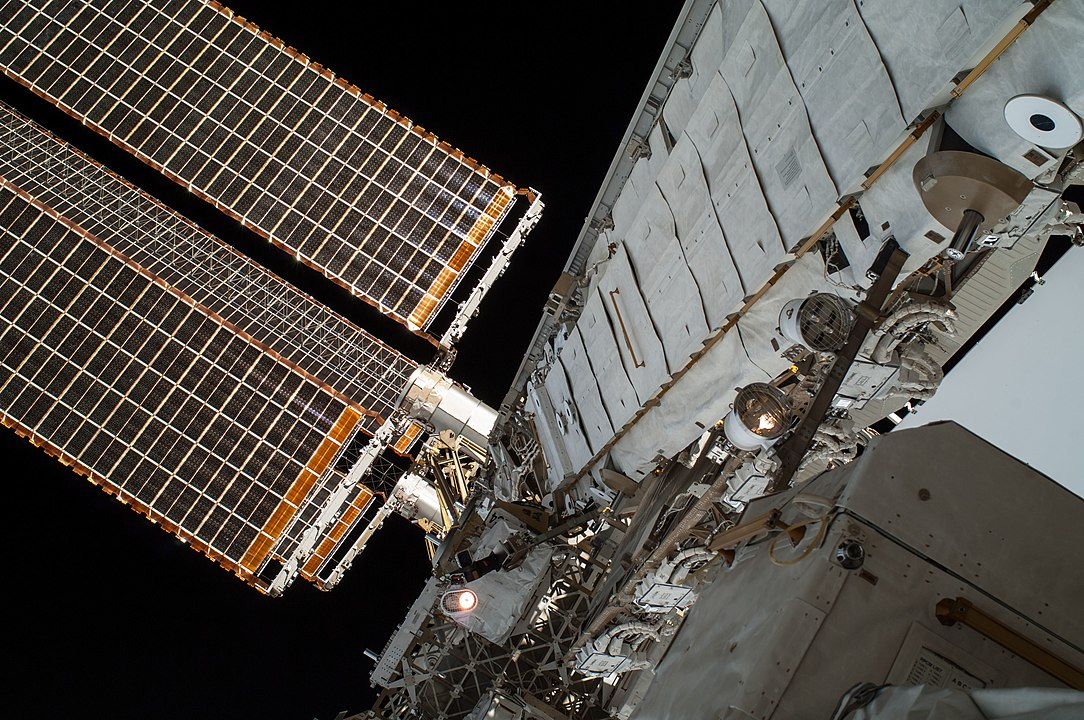
\includegraphics[width=.8\linewidth]{iss-thruss}
	\caption{Integrated truss on the ISS}
	\label{fig:itruss}
\end{figure}

\begin{figure}[H]
	\begin{subfigure}{.5\textwidth}
		\centering
		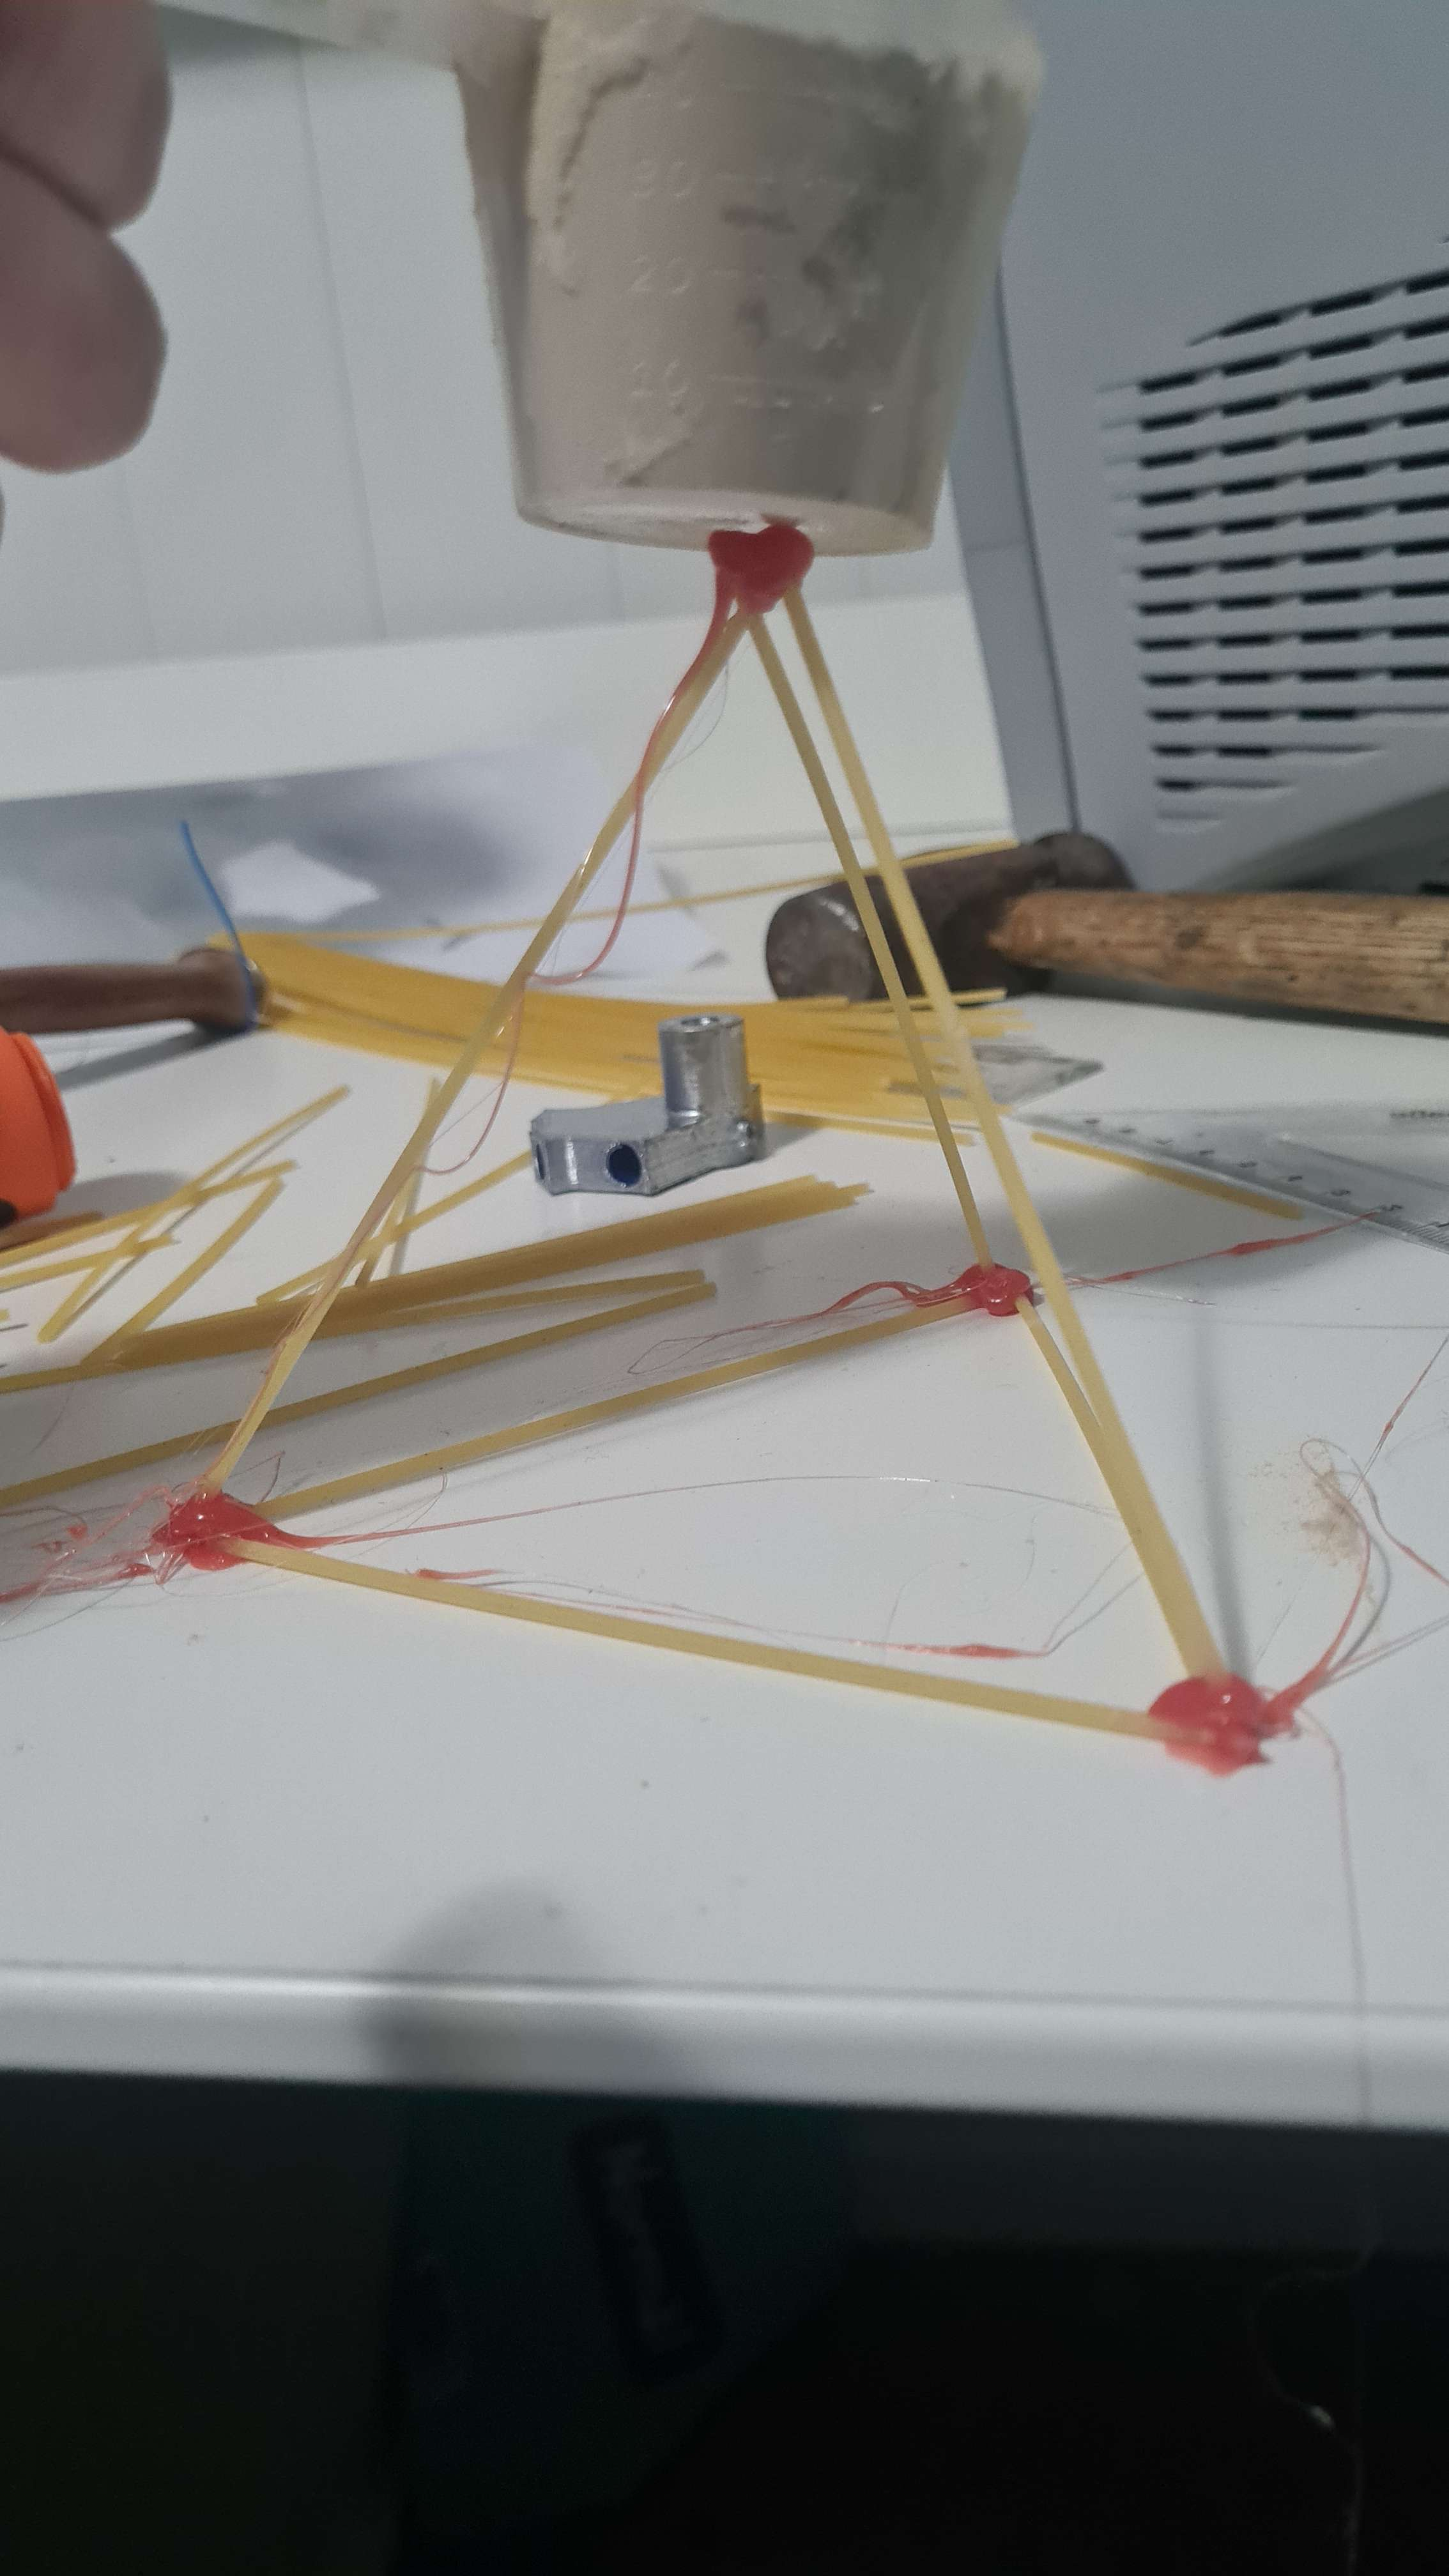
\includegraphics[width=\subimgw,trim={0 20cm 0 0},clip]{tetrehedra-a}
		\caption{Compression buckle isomorphism}

		\label{fig:tetrehedra:a}
	\end{subfigure}%
	\begin{subfigure}{.5\textwidth}
		\centering
		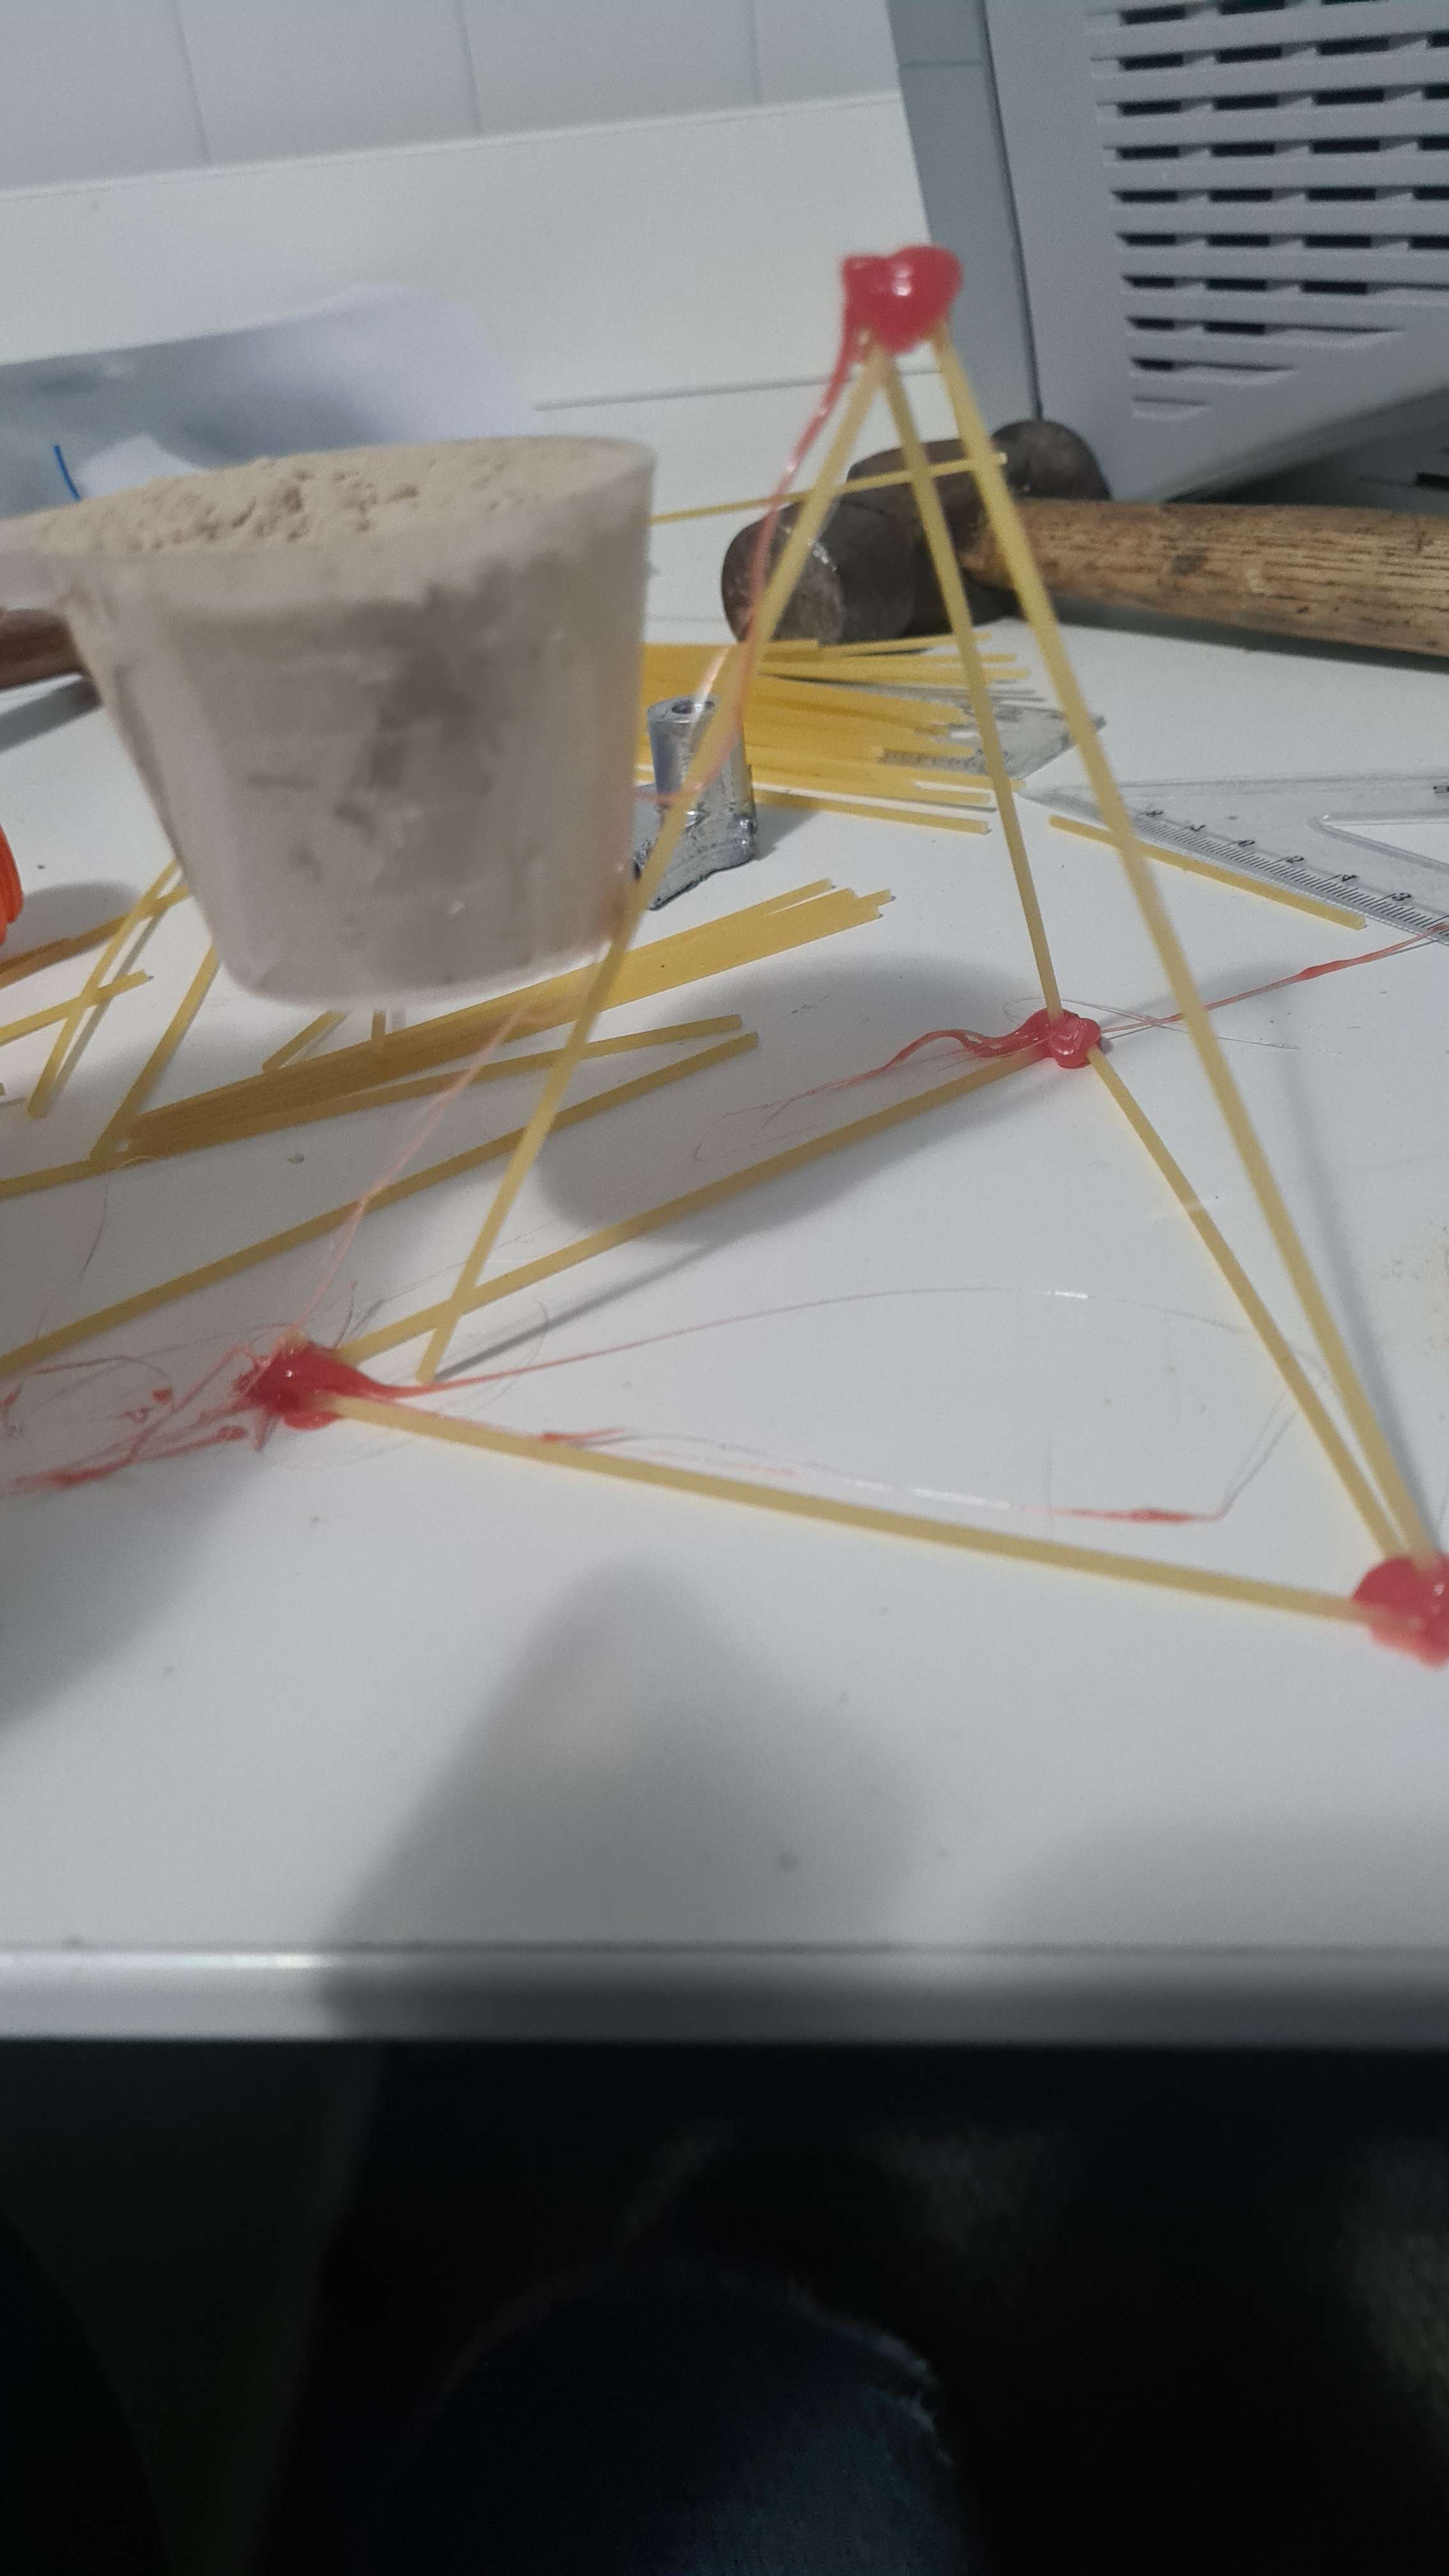
\includegraphics[width=\subimgw,trim={0 20cm 0 0},clip]{tetrehedra-b}
		\caption{Buckle force direction of tetrahedron}

		\label{fig:tetrehedra:untranslated}
	\end{subfigure}

	\caption{Tetrahedron}
	\label{fig:tetrehedra}
\end{figure}

A quad-pyramid has loses a lot of the disadvantages of the isosceles triangle since it is not supported by the other triangles for a more equal force balancing. In bridge building situations this is a lot more of a practical structure than the tetrahedron. This is based on the fact that you can actually build a structural road bellow a pyramid such as this. One can see an example of a quad-pyramid we constructed in Figure \ref{fig:pyramid}.

\begin{figure}[H]
	\begin{subfigure}{.5\textwidth}
		\centering
		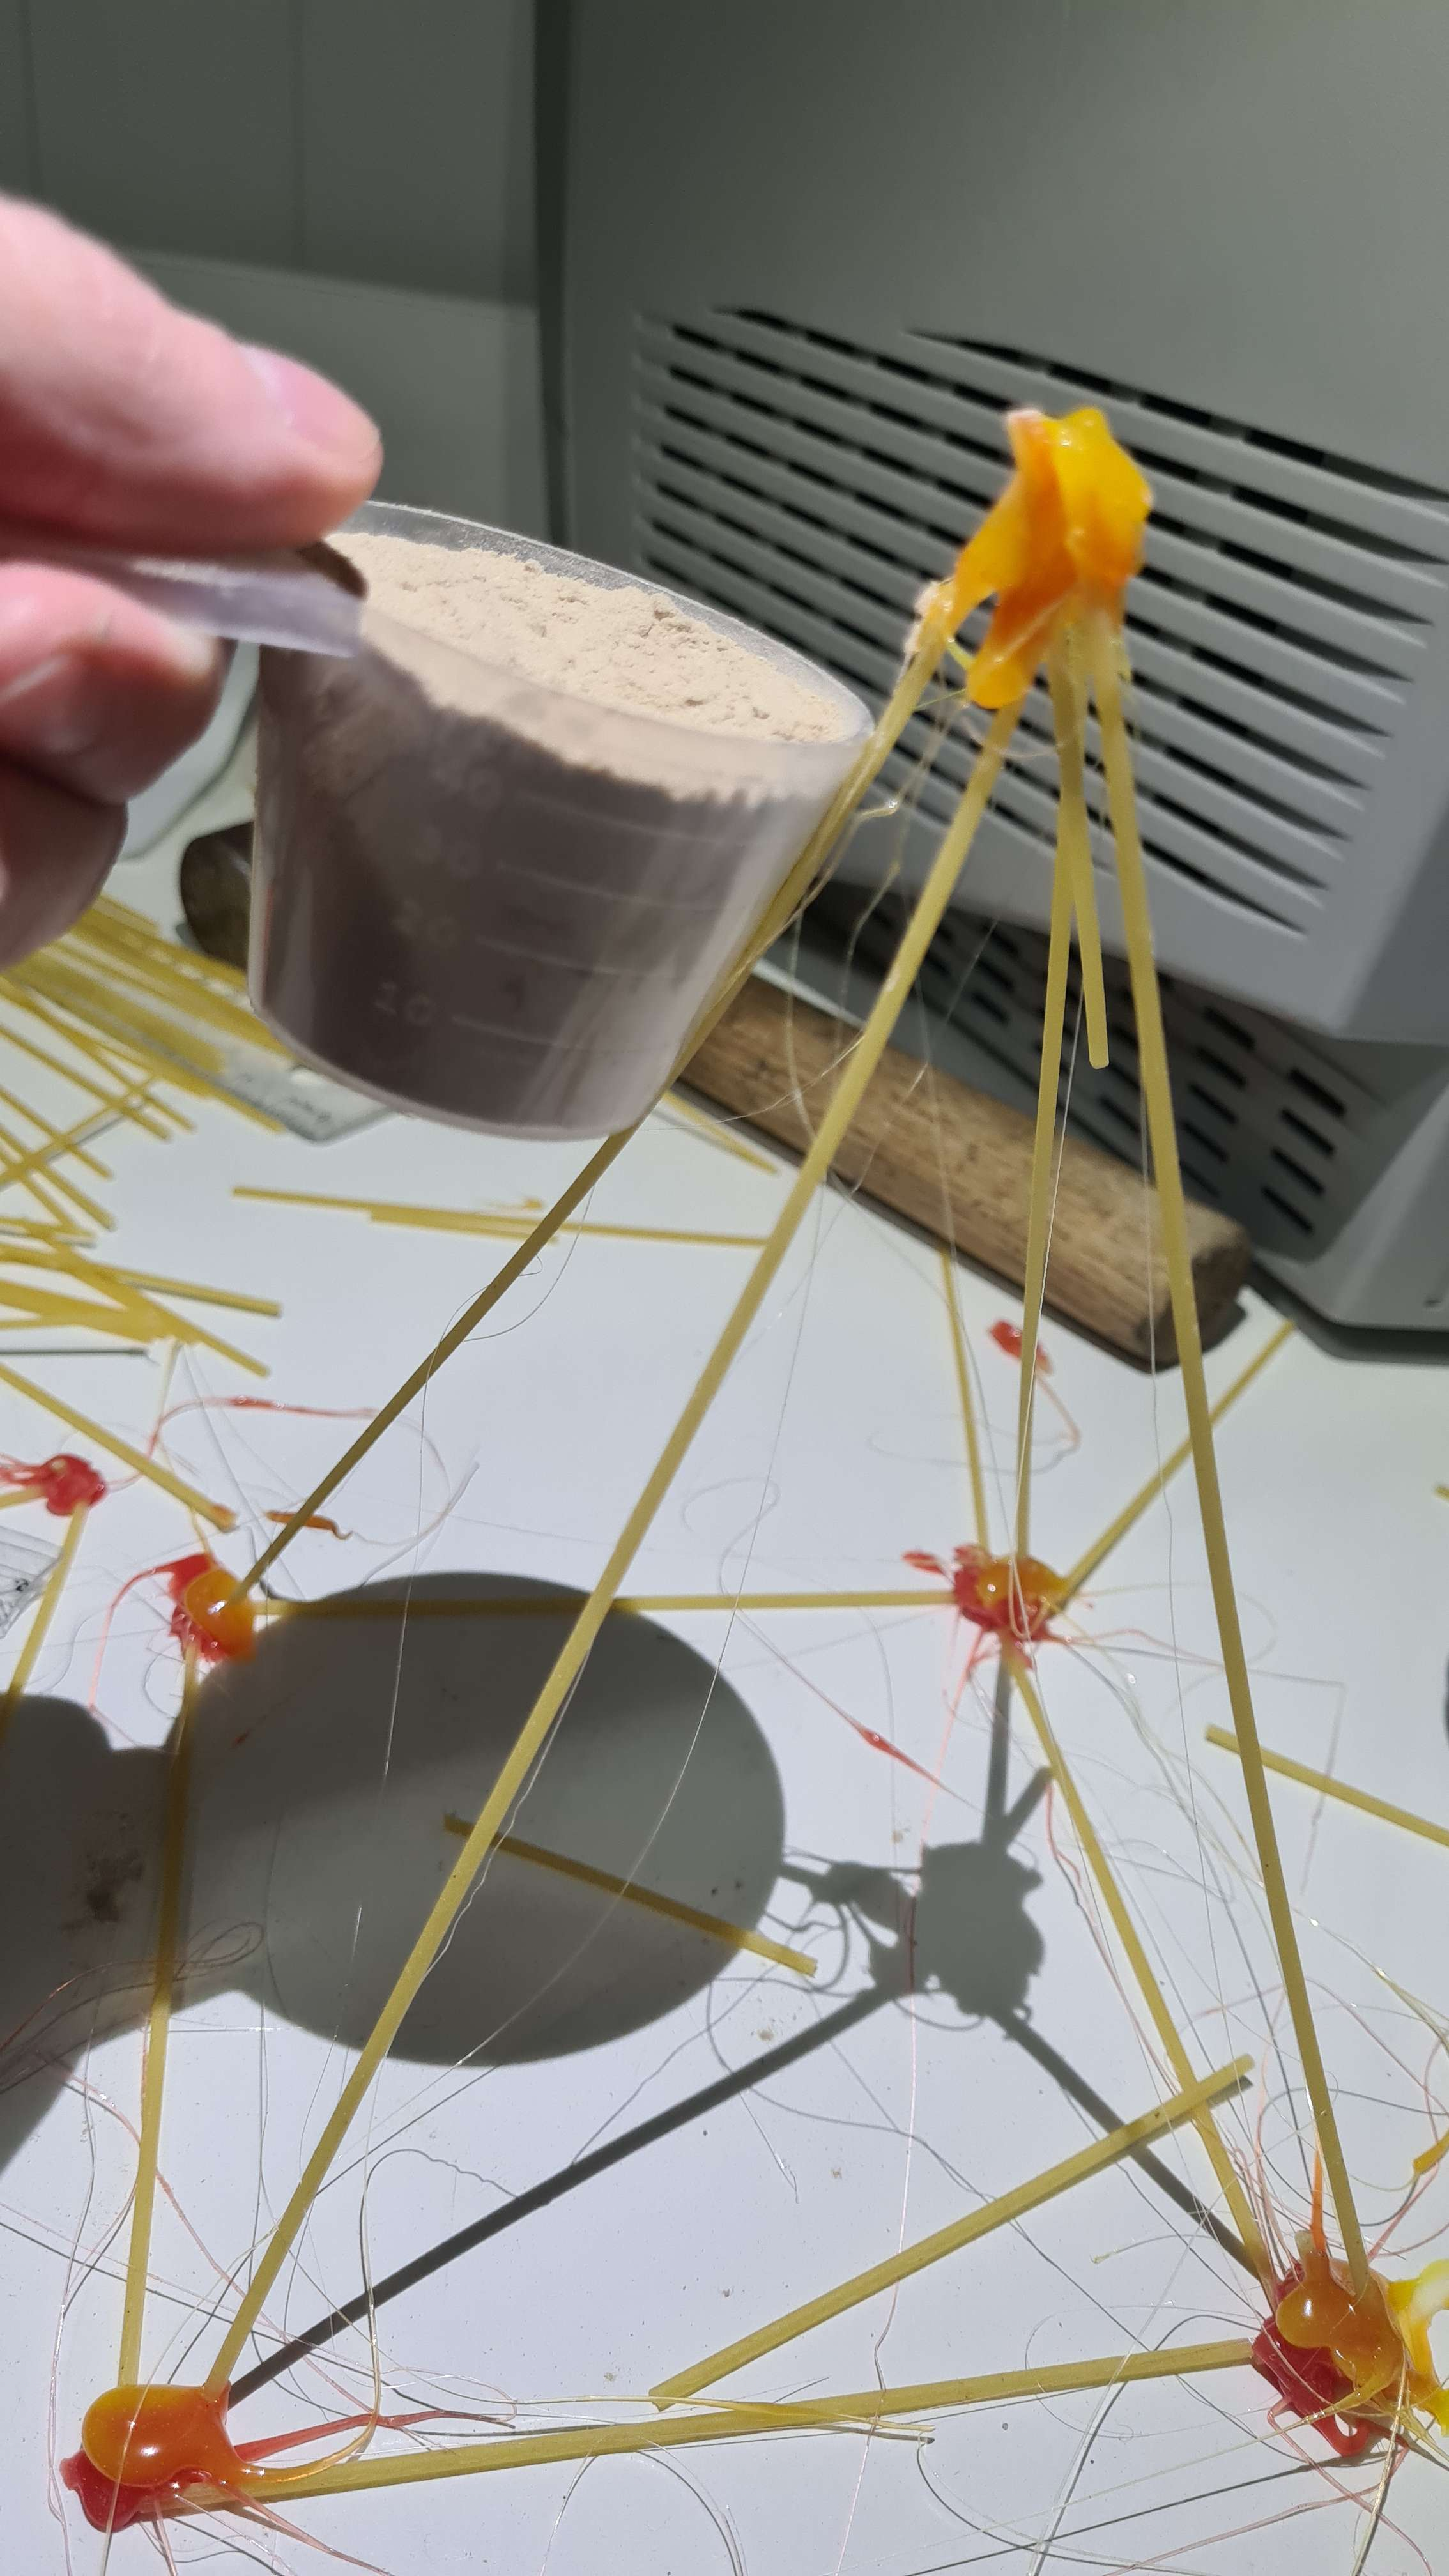
\includegraphics[width=\subimgw]{pyramid-a}

		\caption{Compression and buckle}
		\label{fig:pyramid:a}
	\end{subfigure}%
	\begin{subfigure}{.5\textwidth}
		\centering
		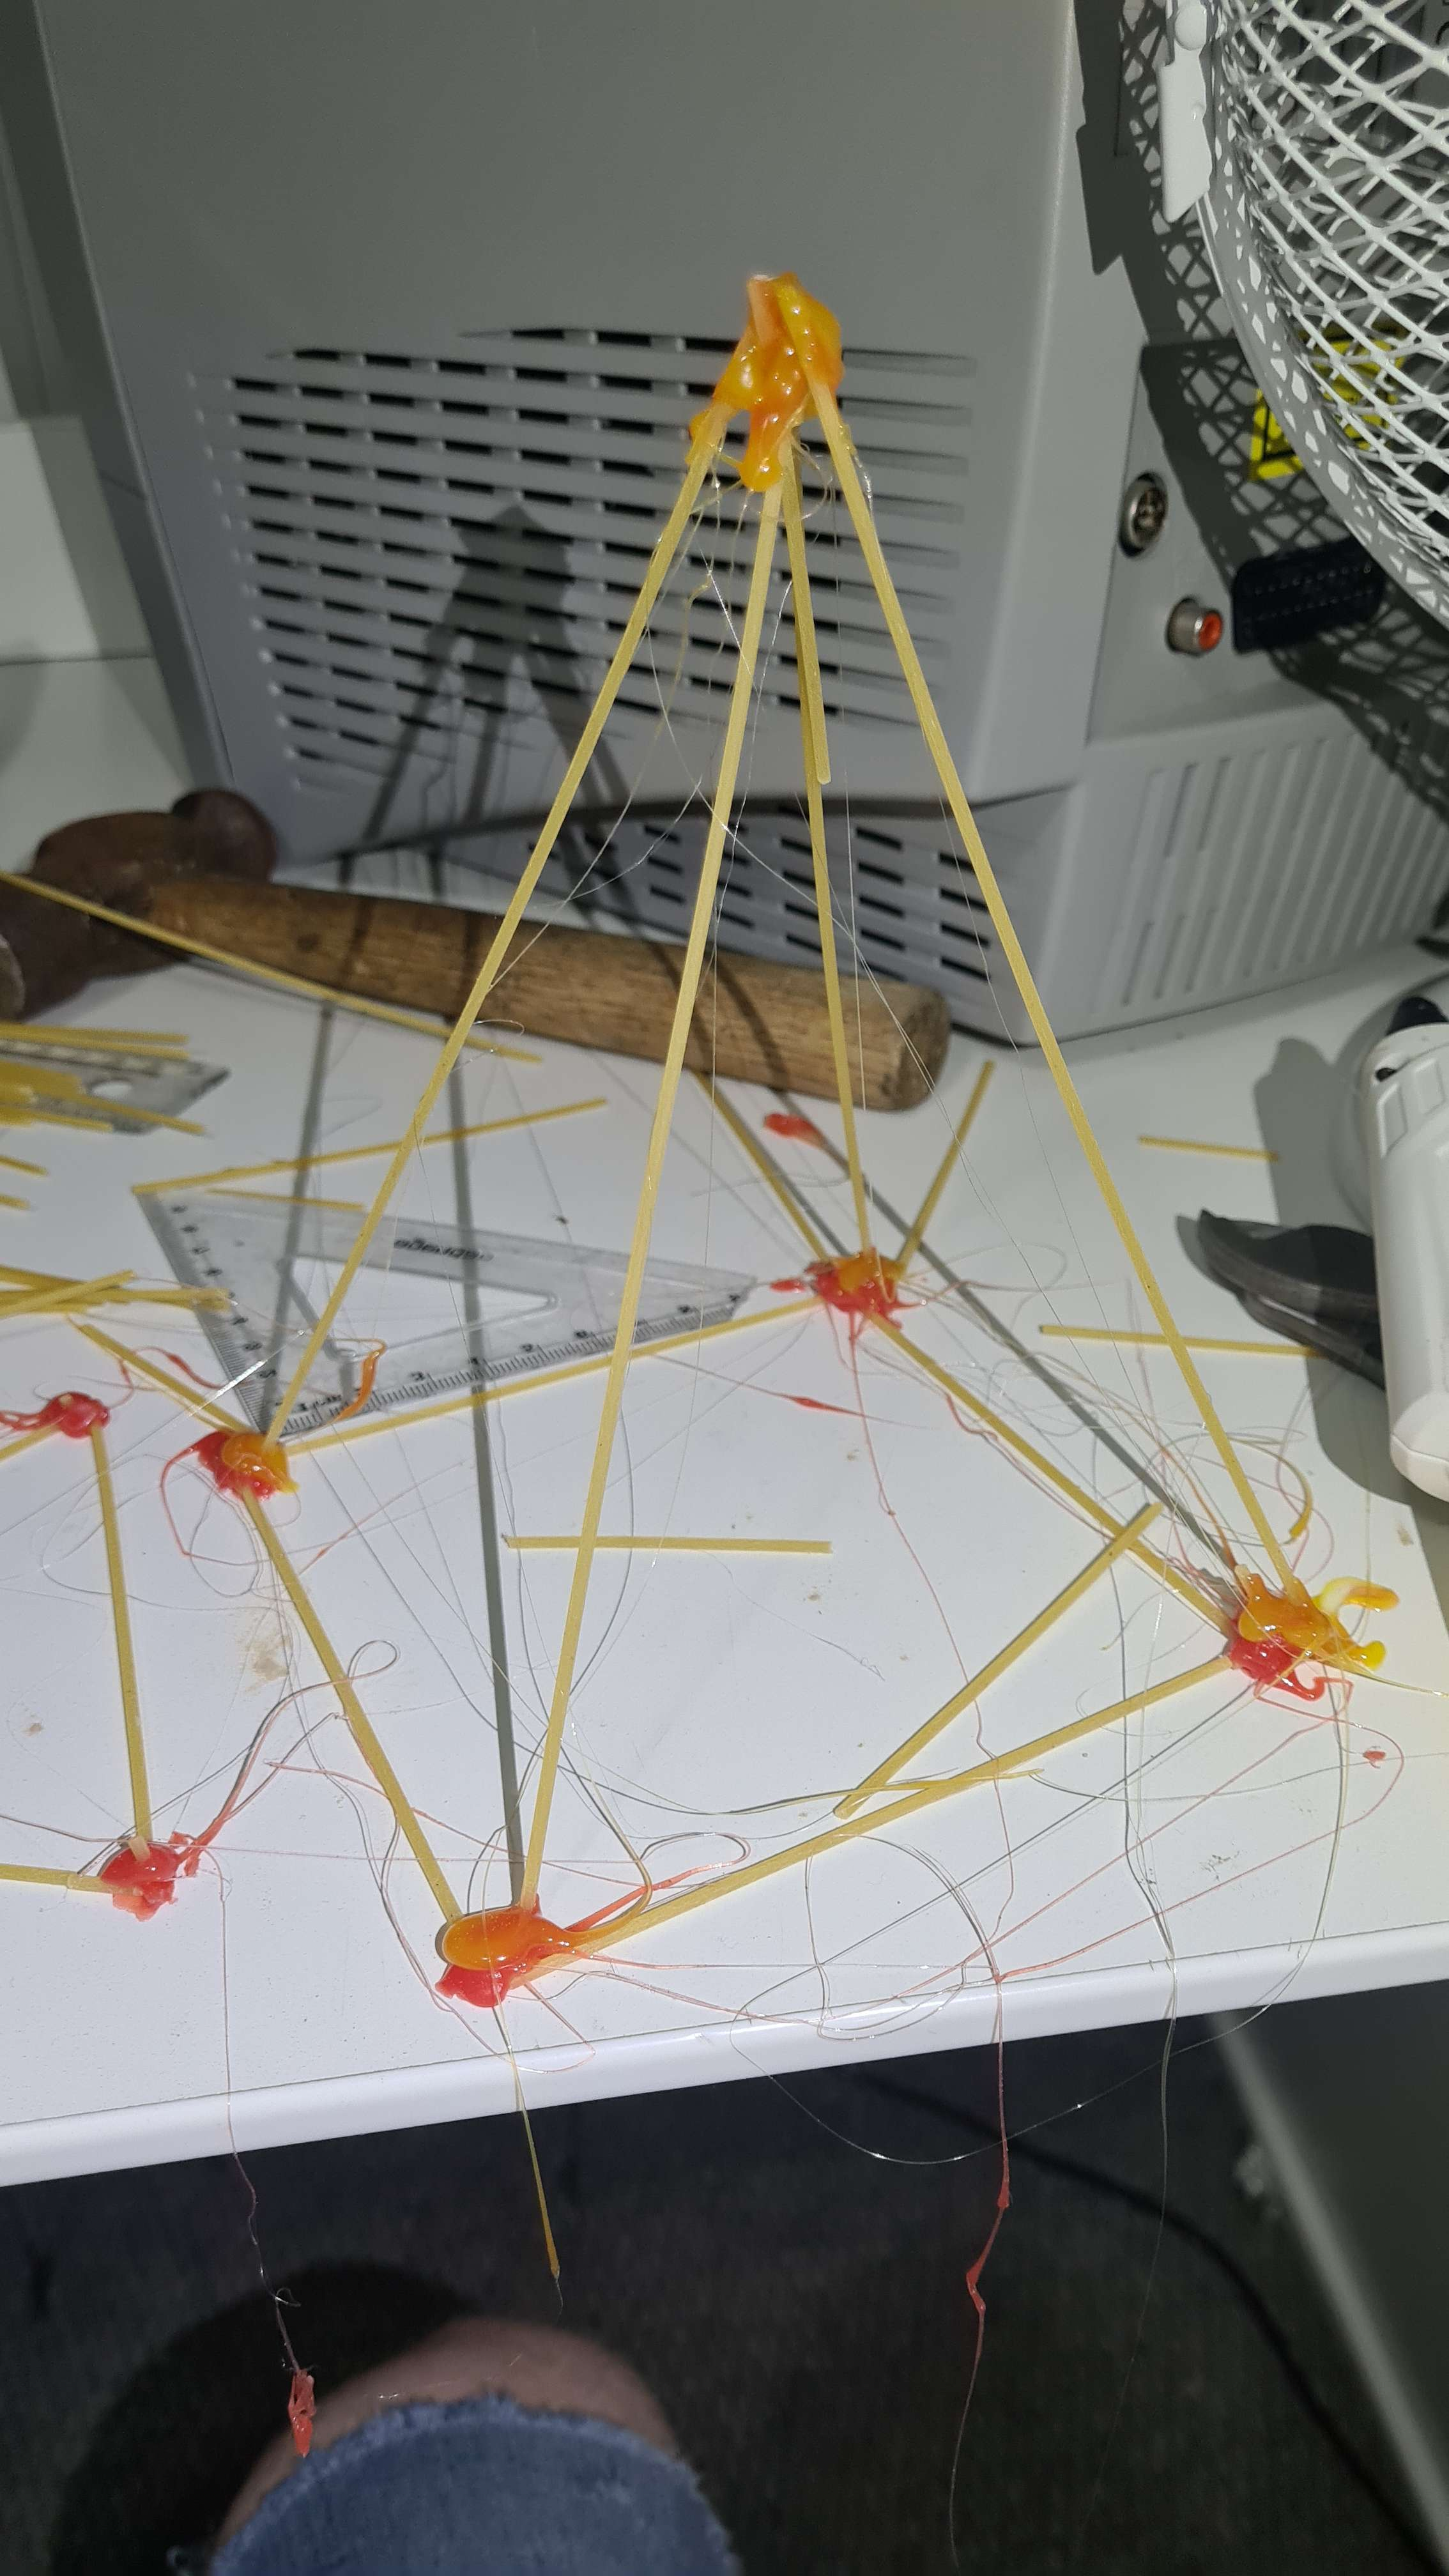
\includegraphics[width=\subimgw]{pyramid-untranslated}

		\caption{Lack of translation}
		\label{fig:pyramid:untranslated}
	\end{subfigure}

	\caption{Quad-pyramid}
	\label{fig:pyramid}
\end{figure}

The cube is the weakest form since any force will lead to a plane translation of the cube. This form of deformation is unacceptable for a truss bridge such as the one we are constructing and hence cannot be used within the bridge. To see a plane translated cube inspect Figure \ref{fig:cube:a} and for its identity seek Figure \ref{fig:cube:untranslated}

\begin{figure}[H]
	\begin{subfigure}{.5\textwidth}
		\centering
		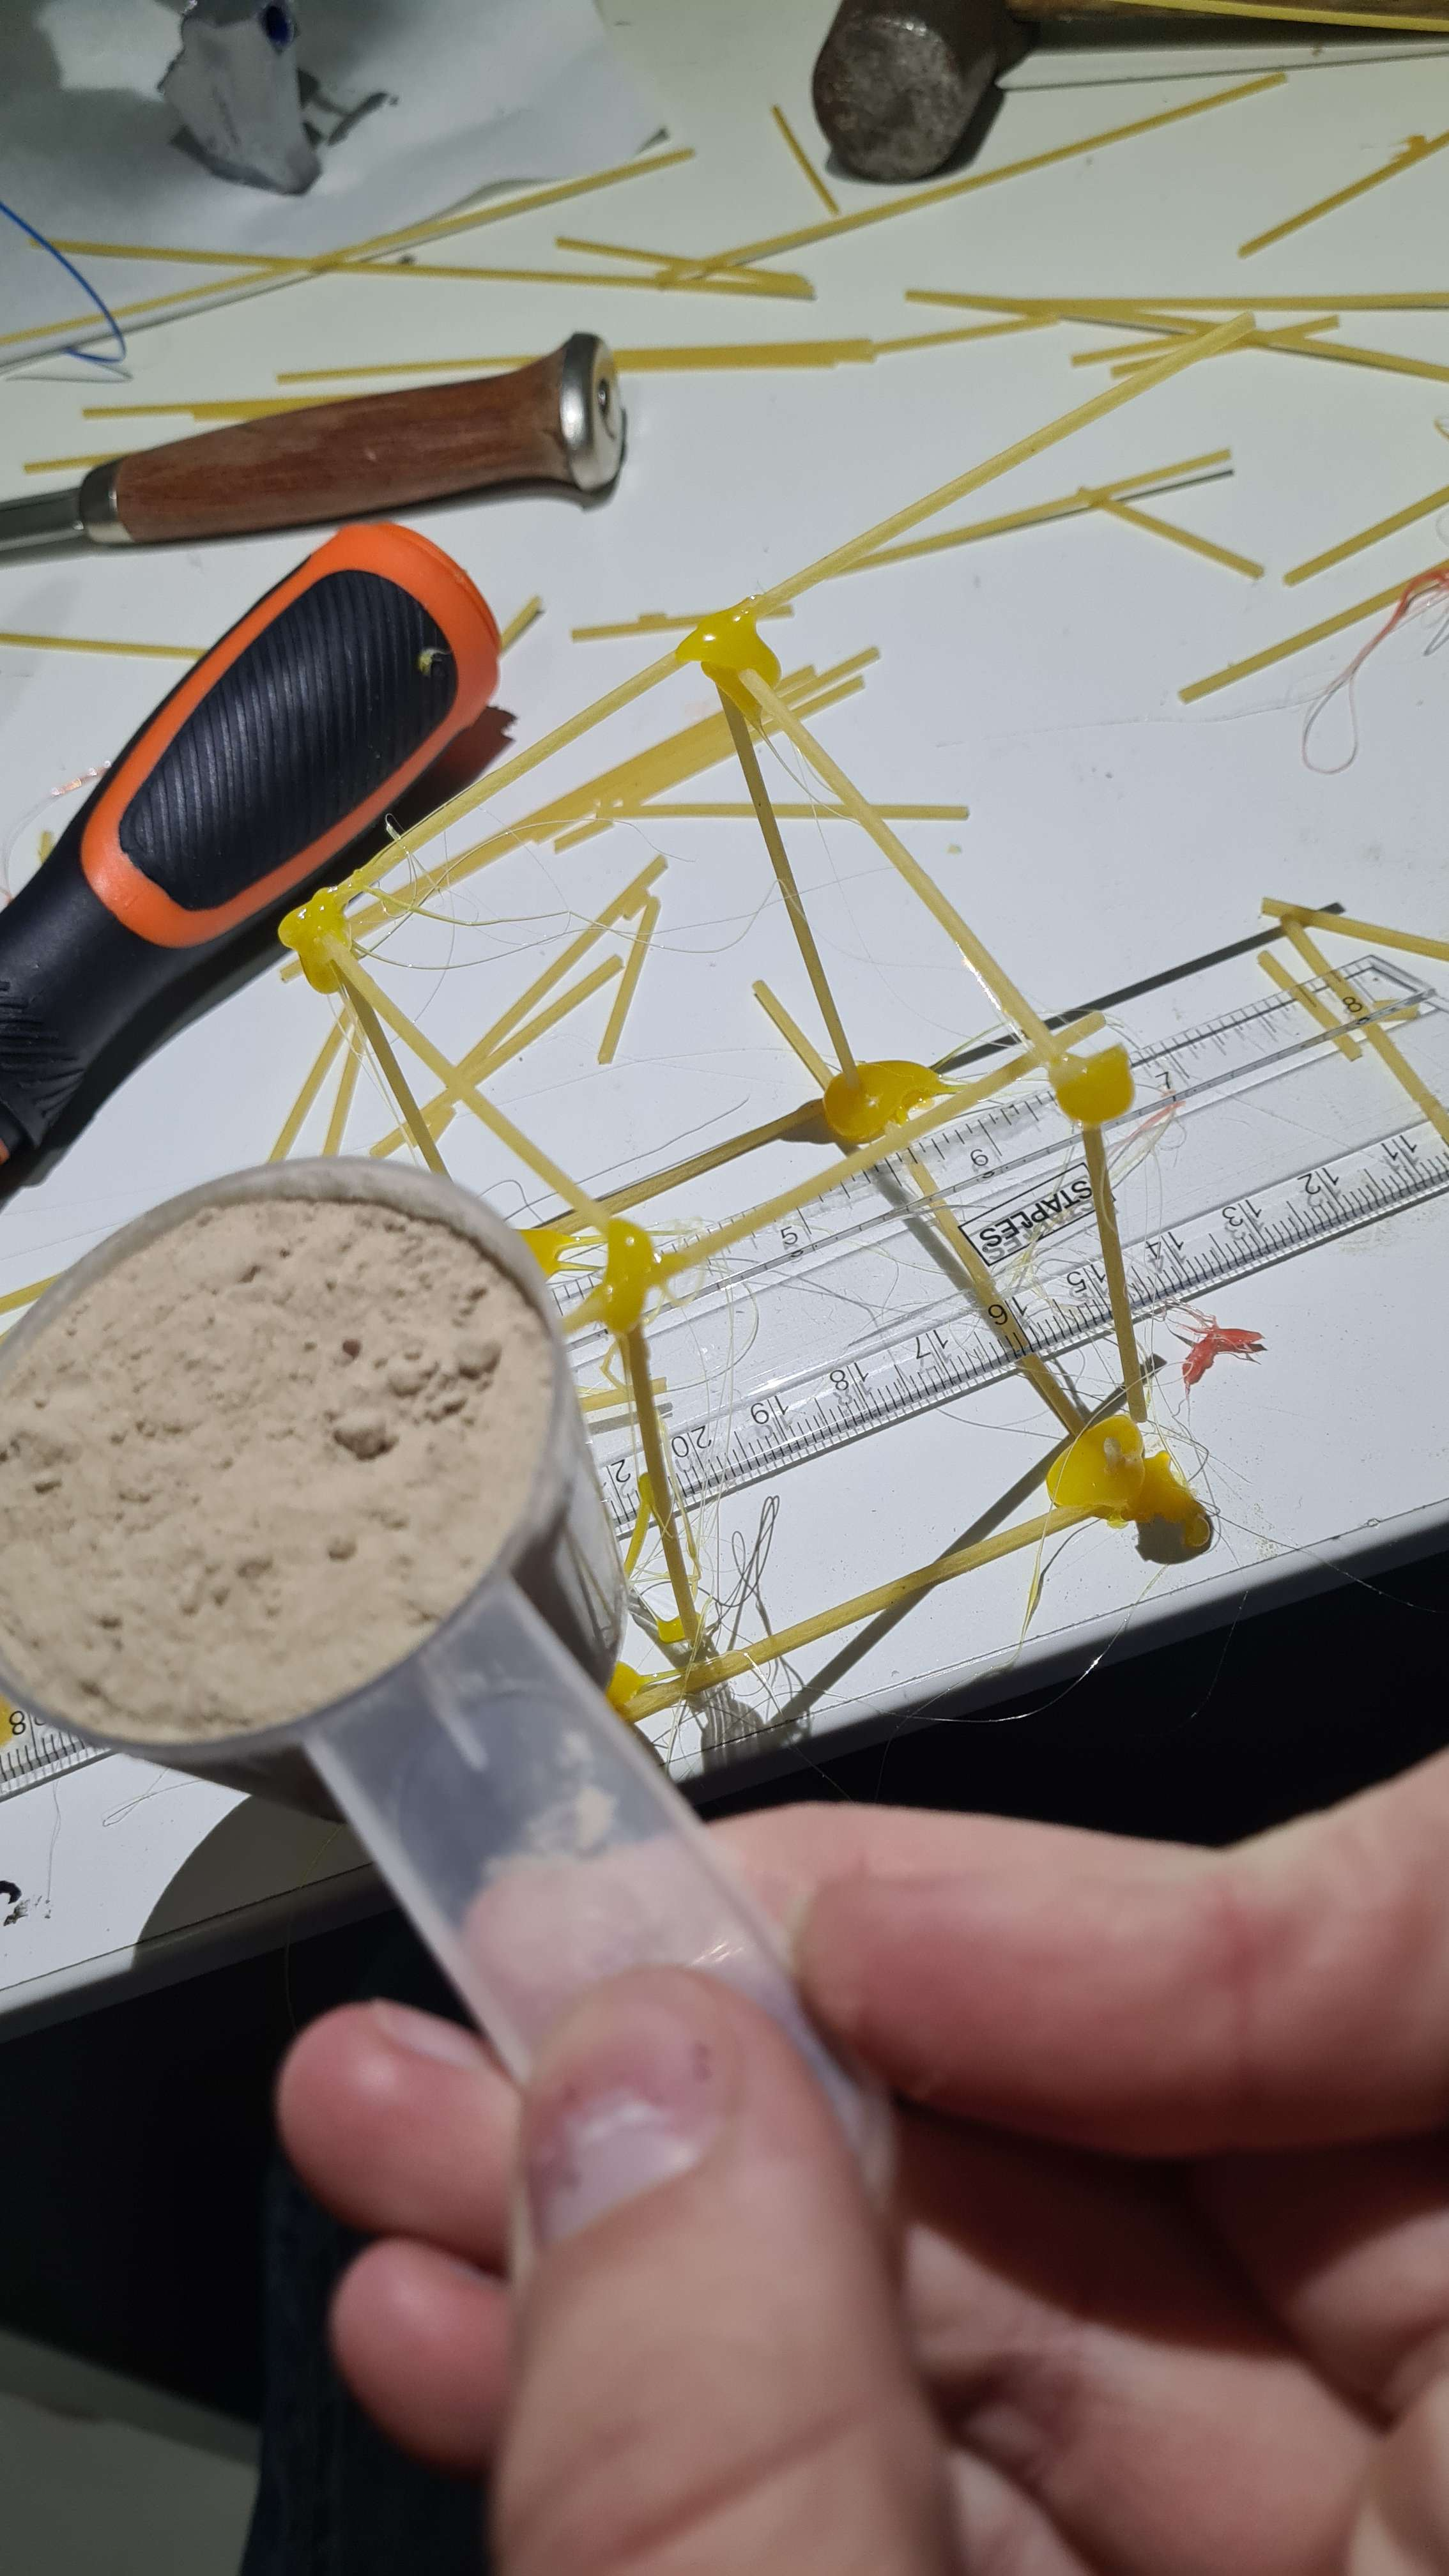
\includegraphics[width=\subimgw]{cube-a}

		\caption{Cube with plane translation}
		\label{fig:cube:a}
	\end{subfigure}%
	\begin{subfigure}{.5\textwidth}
		\centering
		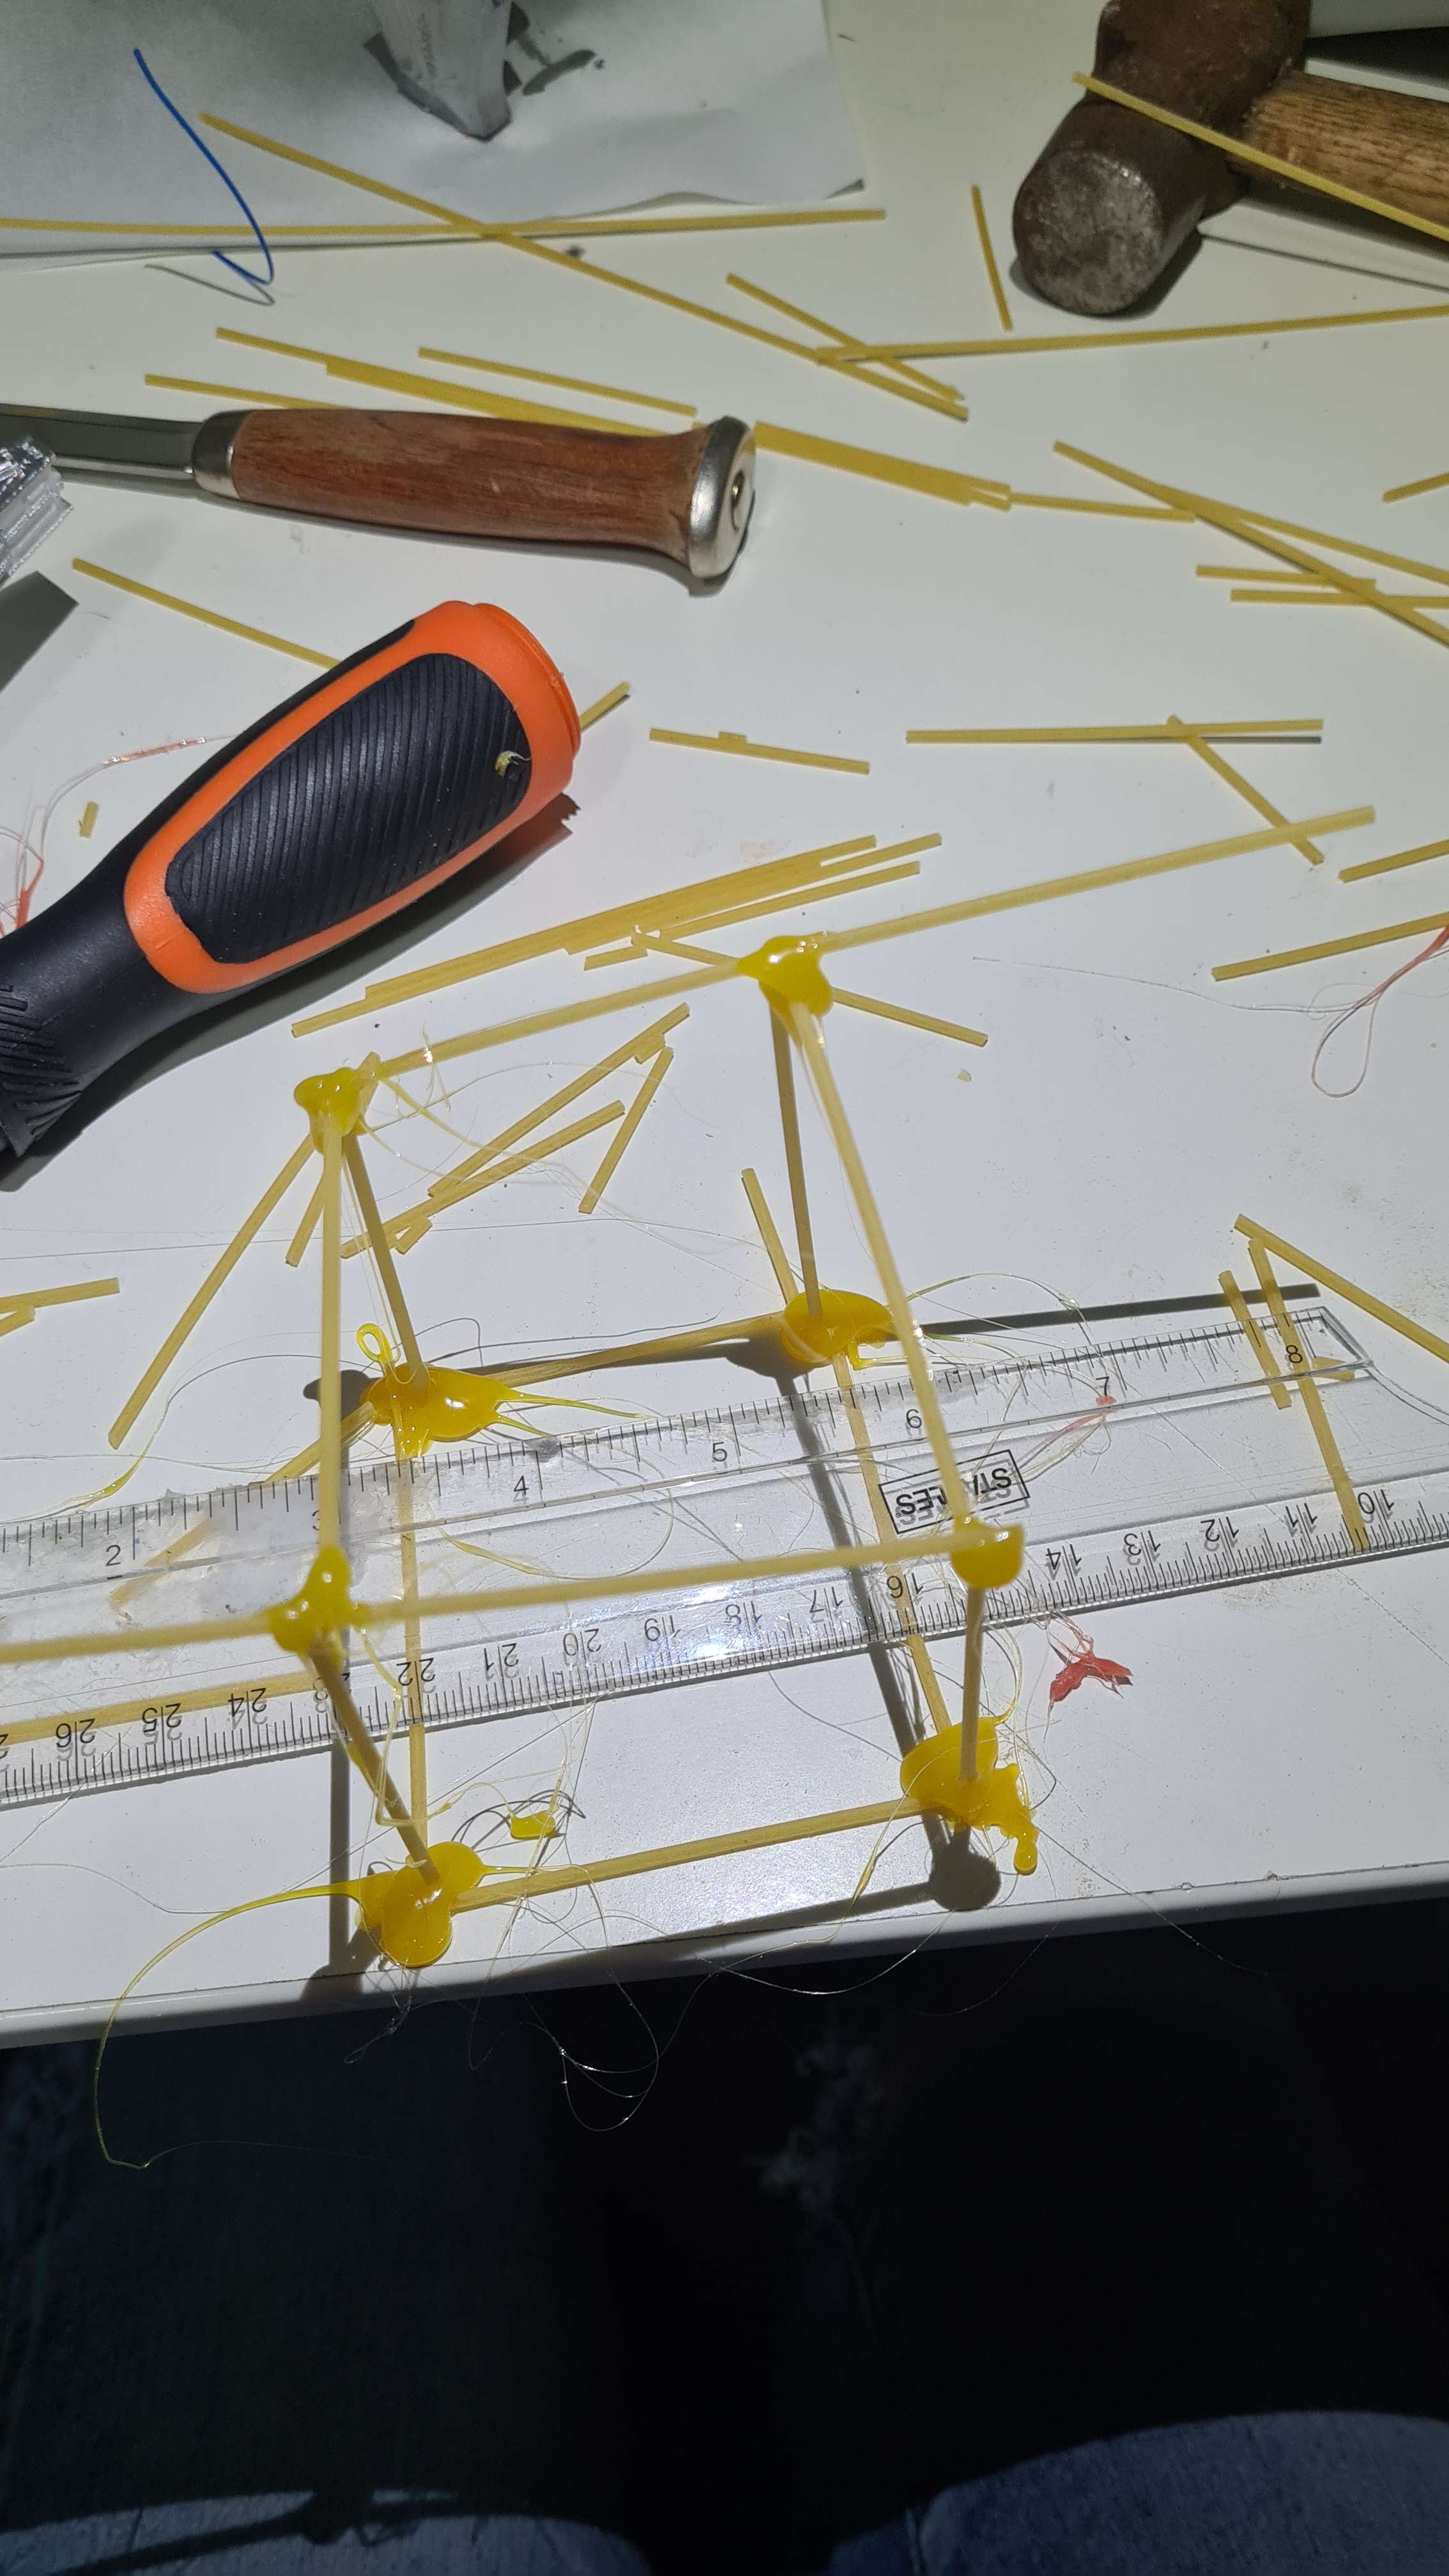
\includegraphics[width=\subimgw]{cube-untranslated}

		\caption{Cube without plane translation}
		\label{fig:cube:untranslated}
	\end{subfigure}

	\caption{Cube}
	\label{fig:cube}
\end{figure}

\section{Task 2}

% Task 2: Forholds-ligningen og bru-modellens dimensjoner

% I forholds-likningen nedenfor er størrelsene 𝐵, 𝐿 og 𝐻 bruens virkelige bredde, lengde og fri høyde. I denne taskn setter vi 𝐵=8,0 meter og 𝐻=4,5 meter. Størrelsene 𝑏, 𝑙 og ℎ er modellbrua sin bredde, lengde og fri høyde. Størrelsen 𝑋 er målestokken. Altså: én cm på modellbrua er 𝑿 cm på den virkelige brua. 𝑏𝐵=𝑙𝐿=ℎ𝐻=1𝑋

% 2A: Velg en passende verdi for 𝑙, 𝑏 eller ℎ, og regn ut målestokken 𝑋 til modellbrua. Bruk målestokken til å regne ut de ukjente verdiene nedenfor. I besvarelsen skal dere kort vise hvordan dere regnet ut alle tallene. Dere kan for eksempel ved å vise svarene og kodene fra Excel eller Python.

% Bredde: 𝑏 cm Lengde: 𝑙 cm eksklusiv landkar.

% Bredde kjørebane: 𝑏𝐾 cm Gang- og sykkelsti: 𝑏𝐺𝑆 cm på hver side.

% Fri høyde: ℎ cm.

% 2B: Vi har flere forskjellige modell-materialer tilgjengelig. Regn ut modell-materialenes virkelige størrelse og modellbrua sin størrelse i henhold til målestokken dere har valgt.

% I besvarelsen skal dere fylle ut tallene som mangler i tabellen nedenfor. Dere må vise hvordan dere regnet ut svarene. Dere kan for eksempel løse taskn ved å bruke Excel eller Python, og vise kodene.

In this task, you were supposed to calculate a scale for the group's model bridge. This is done by using the real size of the bridge and dividing it by our selected scale.

\subsection{a}

We use the length of the bridge to calculate the scale. The length of the model bridge is $80\mathrm {cm} = 0.80\mathrm m$, the real bridge is $28\mathrm m$ (class A). This gives us $\frac {25} {.8} = 35$.

\subsection{b}

We have split the table into two tables. There is the materials table as Figure \ref{fig:tomr} and the dimensions table as Figure \ref{fig:todr}

\begin{figure}[H]
	\centering
	\begin{tabular}{|c|c|c|}
		\hline
		Material     & Model scale                          & IRL Scale                                \\
		\hline
		Bambuspinner & $3\mathrm{mm} \times 28 \mathrm{cm}$ & $105\mathrm{mm} \times 980 \mathrm{cm}$  \\
		Bambuspinner & $4\mathrm{mm} \times 40 \mathrm{cm}$ & $140\mathrm{mm} \times 1400 \mathrm{cm}$ \\
		Bambuspinner & $6\mathrm{mm} \times 40 \mathrm{cm}$ & $210\mathrm{mm} \times 1400 \mathrm{cm}$ \\
		Trekule      & $15\mathrm{mm}$                      & $525\mathrm{mm}$                         \\
		Trekule      & $20\mathrm{mm}$                      & $700\mathrm{mm}$                         \\
		Trekule      & $25\mathrm{mm}$                      & $875\mathrm{mm}$                         \\
		\hline
	\end{tabular}
	\caption{Table of material re-scales}
	\label{fig:tomr}
\end{figure}

\begin{figure}[H]
	\centering

	\begin{tabular}{|c|c|c|}
		\hline
		dimension         & Model Scale      & IRL scale      \\
		\hline
		Length            & $80 \mathrm{cm}$ & $28 \mathrm m$ \\
		Width             & $23 \mathrm{cm}$ & $8\mathrm m$   \\
		Width carriageway & $17 \mathrm{cm}$ & $6\mathrm m$   \\
		Width pavement    & $3  \mathrm{cm}$ & $1\mathrm m$   \\
		Free height       & $13 \mathrm{cm}$ & $4.6\mathrm m$ \\
		\hline
	\end{tabular}

	\caption{Table of dimension re-scale}
	\label{fig:todr}
\end{figure}

\section{Task 3}

In task 3 one was supposed to use the scaling one has previously calculated to produce a blueprint. This should be done on paper and we have done this in Figure \ref{fig:paper} but we have also done it in Tikz (Figure \ref{fig:tikz}) and OpenSCAD (Figure \ref{fig:bridge}).

\begin{figure}[H]
	\centering
	\includegraphics[width=.8\linewidth]{frame00000}

	\caption {OpenSCAD dump of bride including a legend of the different measurements.}
	\label{fig:bridge}
\end{figure}

\begin{figure}[H]
	\centering
	\begin{tikzpicture}
		\draw (0,-1.5) rectangle (7,1.5);
		\draw (0,1.5) rectangle (7,2);
		\draw (0,-1.5) rectangle (7,-2);

		\draw (-.3,-1.5)[<->] --node[midway,left]{17cm} (-.3,1.5);
		\draw (-.3,1.5)[<->]  --node[midway,left]{3cm}  (-.3,2);
		\draw (-.3,-1.5)[<->] --node[midway,left]{3cm}  (-.3,-2);
	\end{tikzpicture}
	\caption{Tikz edition}
	\label{fig:tikz}
\end{figure}

\begin{figure}[H]
	\centering
	\begin{subfigure}{.5\textwidth}
		\centering
		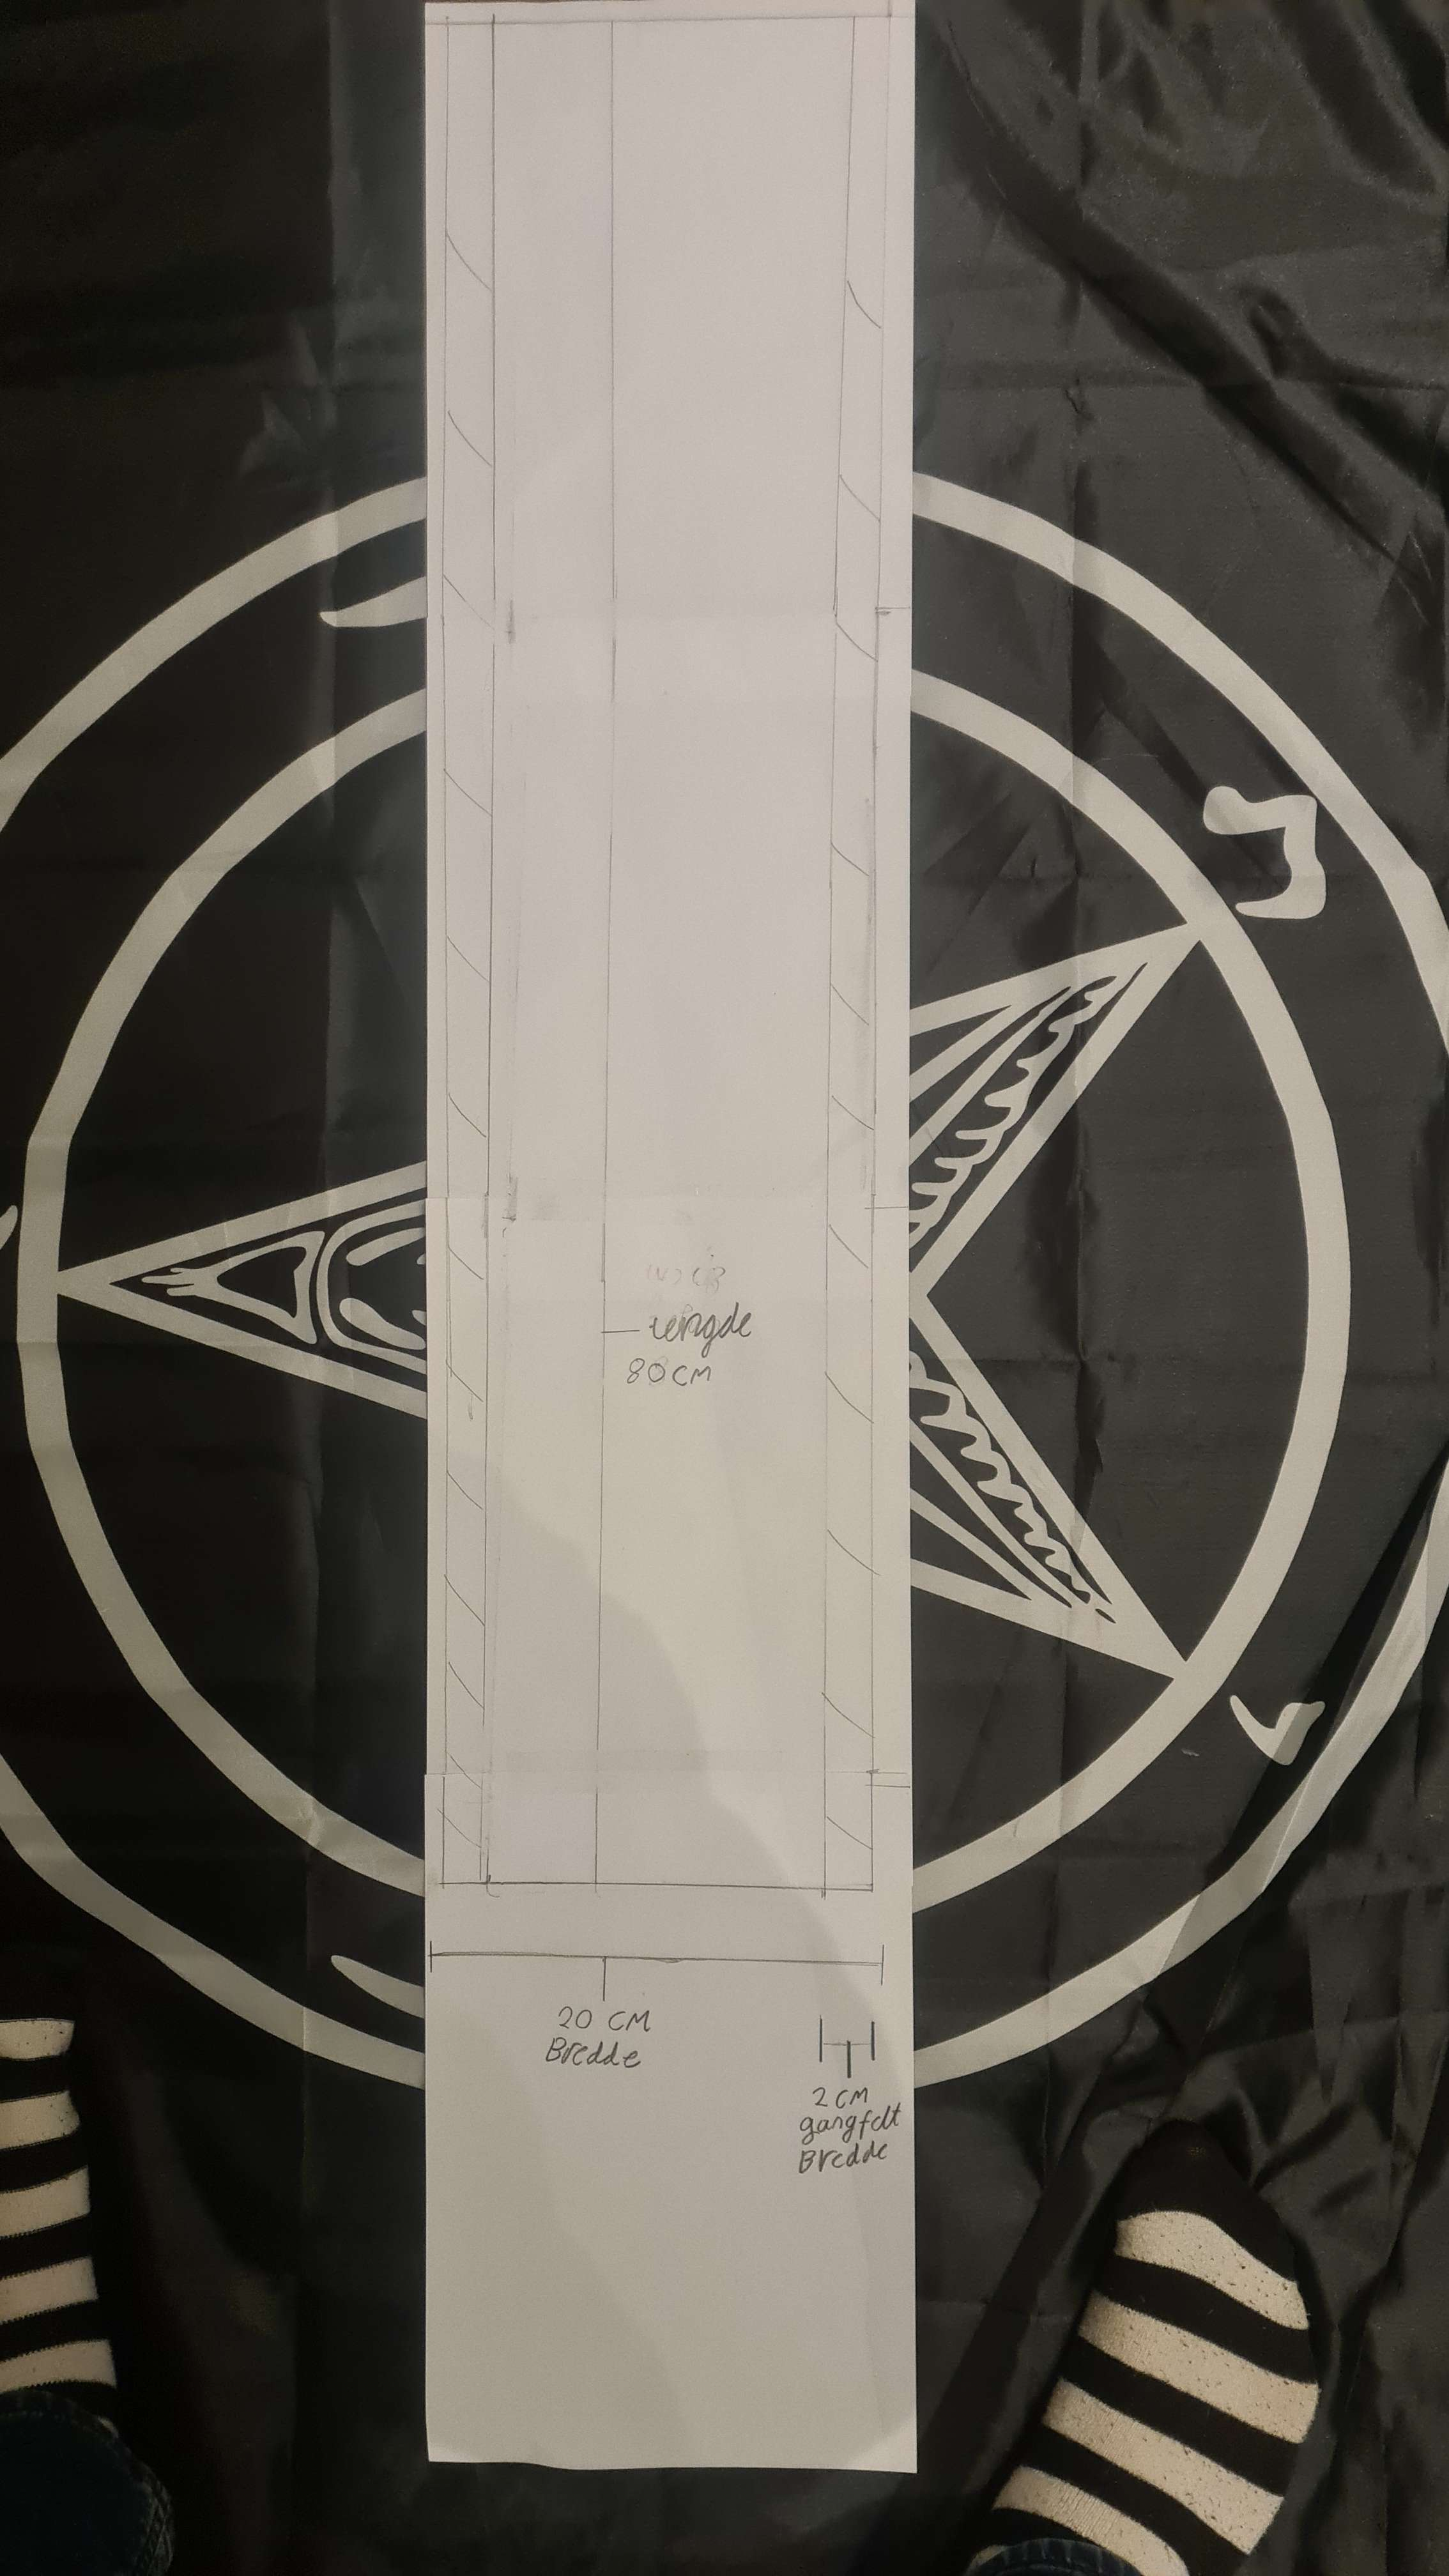
\includegraphics [width=\subimgw]{task-3-far}

		\caption{Far image}
	\end{subfigure}%
	\begin{subfigure}{.5\textwidth}
		\centering
		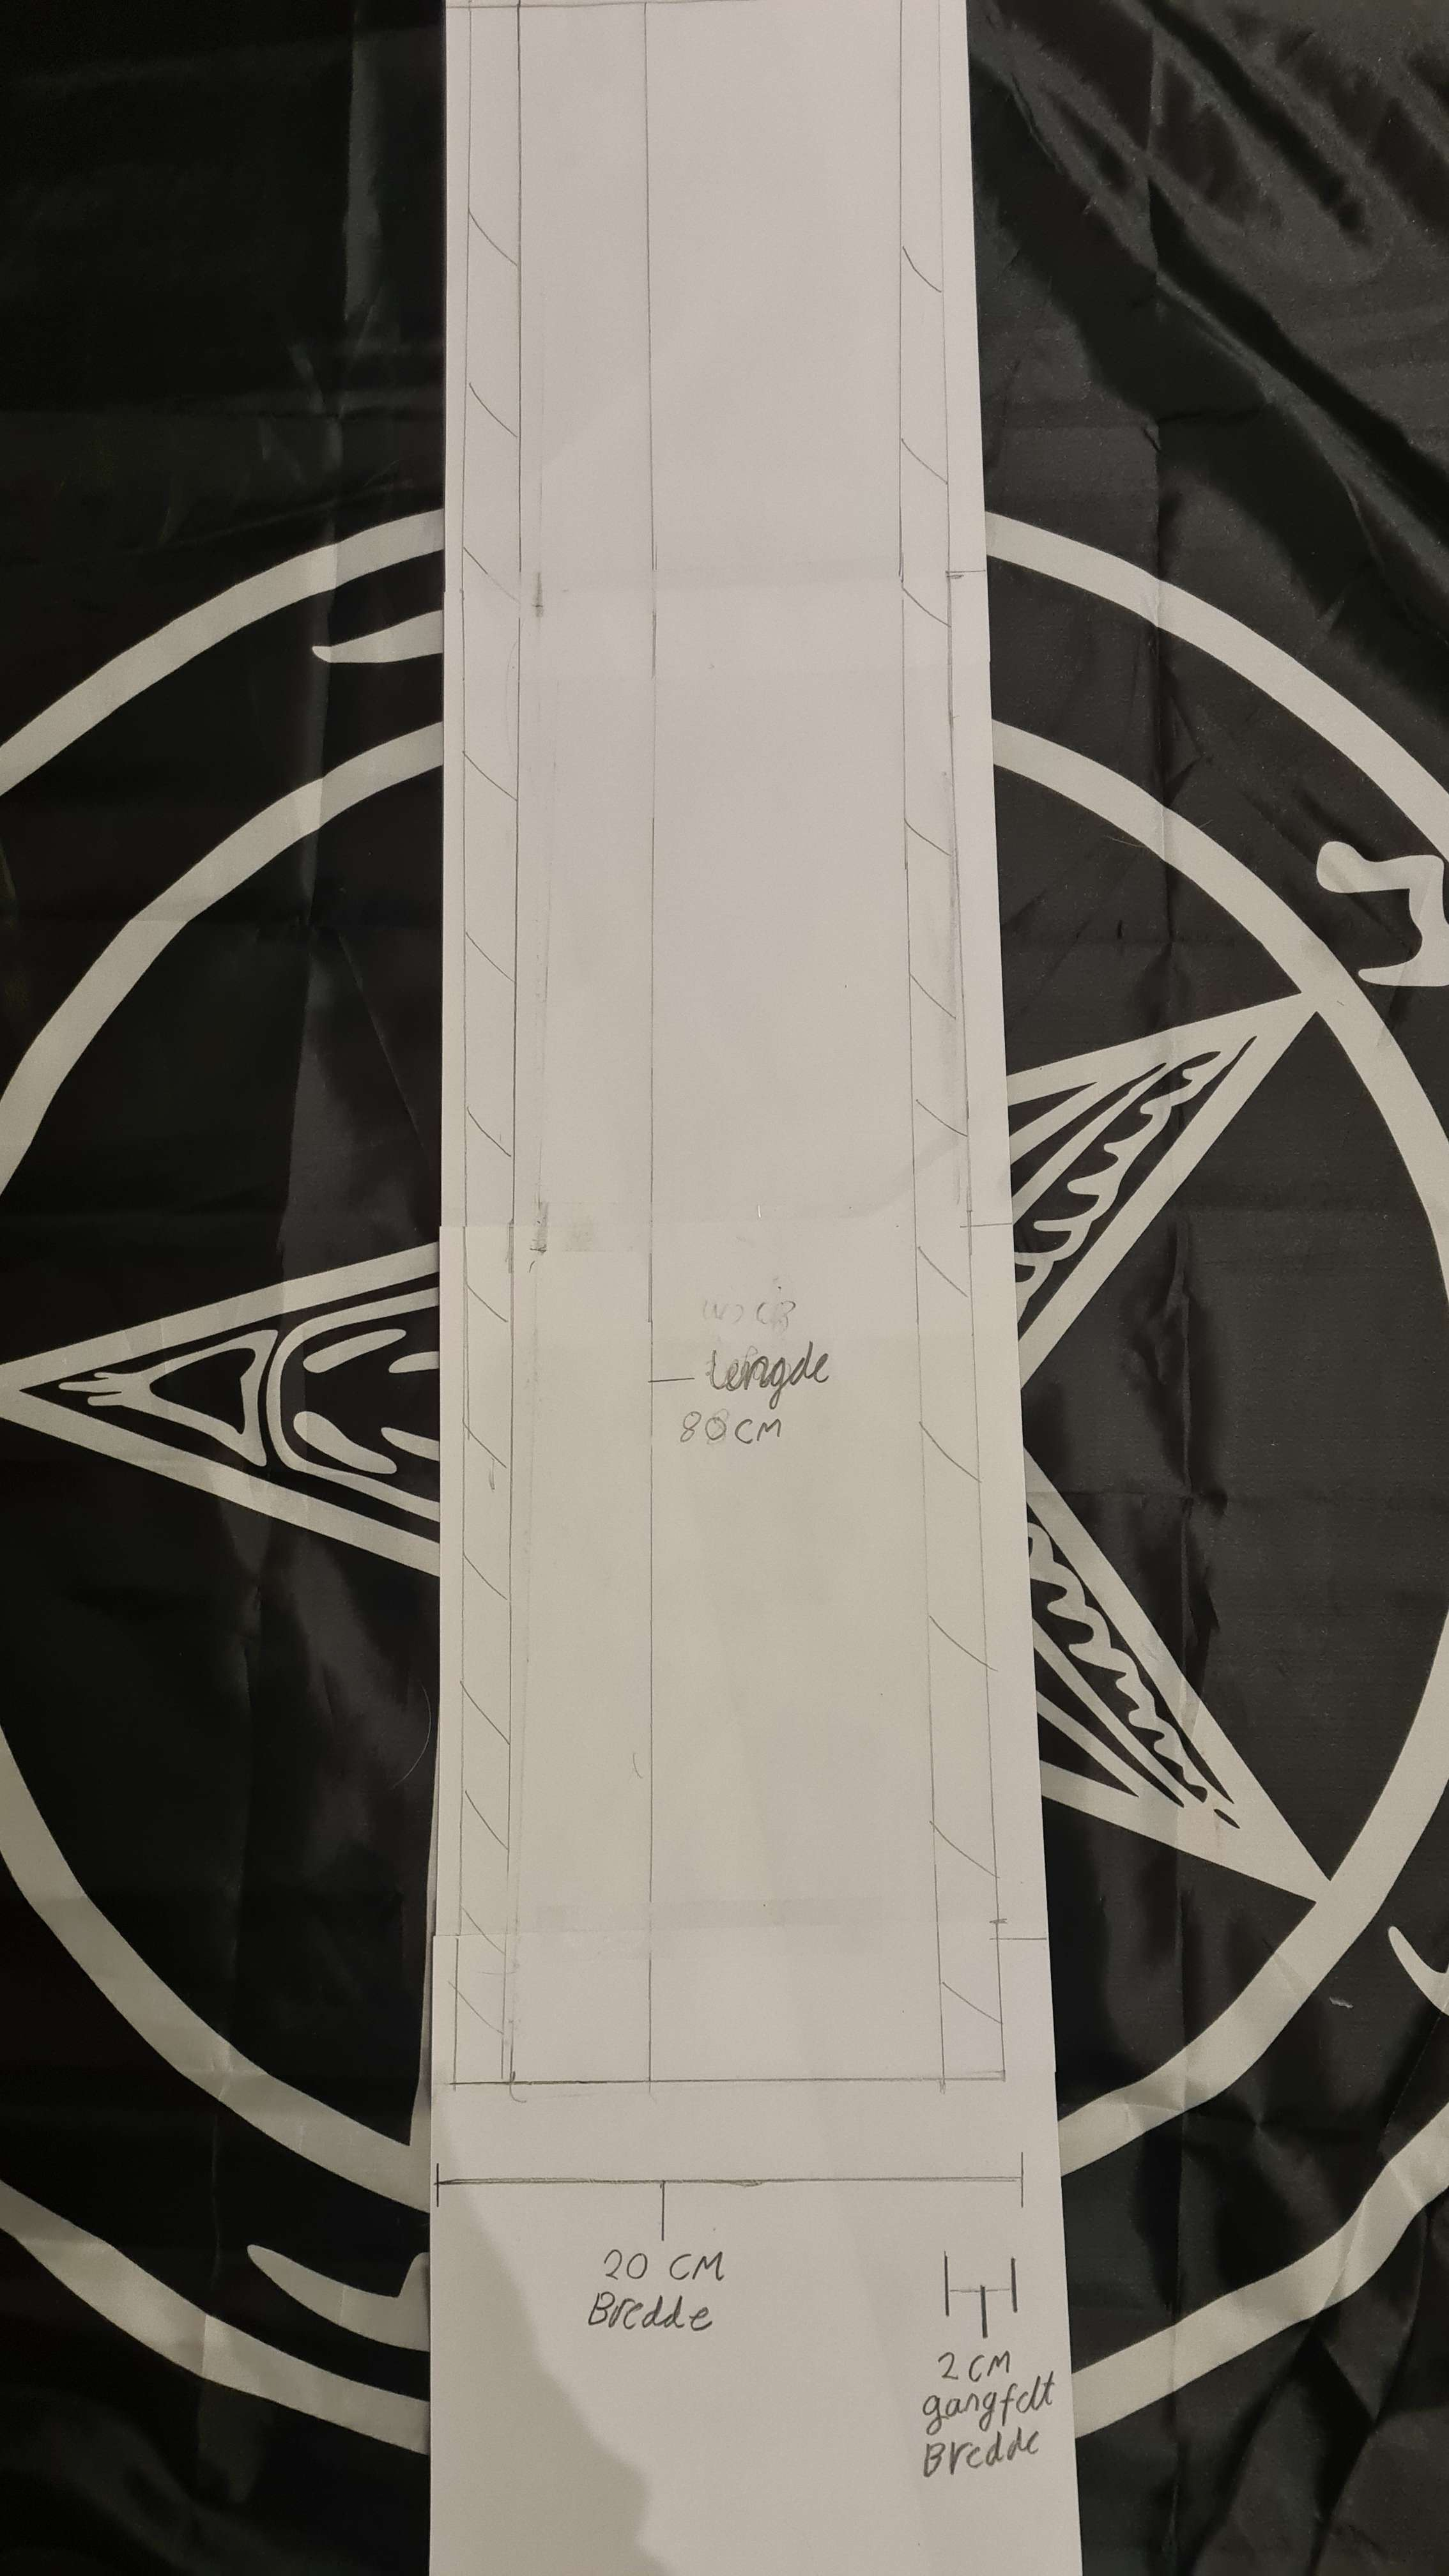
\includegraphics [width=\subimgw]{task-3-near}

		\caption{Near image}
	\end{subfigure}
	\caption{Task 3 paper editions}
	\label{fig:paper}
\end{figure}

\section{Task 4}

We have decided to design our bridge from a few facets of the specification. Primarily we have taken an environmental approach to constructing the bridge but we have also made sure to be able to represent the regions rich history through paying homage to great traditions such as fishing and pride.

The bridge is planned to be a so called energy positive construction. This means that through its long lifespan we wish for it to absorb more $CO_2$ and produce more energy than it was required to construct the bridge. To achieve this we have constructed the bridge out of powerful renewed material such as PLA \cite{wiki:pla}. We have also added solar panels to the bridge which will allow it to resend power back into the electrical grid to for example assist the semiconductor manufacturer.

From a cultural perspective we have incorporate fish and fishing equipment into the bridge. This ranges from adding fish decals (which in this case are 3D printed) to more intricate decorations such as the fishing net on one of the sides of the bridge. This symbolizes the history of fish and fishing in Lofoten over the ages.

We have also painted these fishes silver. This comes from the proximity to the semiconductor manufacturer which we wish to represent in the bridge design.

Other than fishing we have also added a pride aspect to the bridge. This comes from wish to represent all of the diverse inhabitants of the region and to do this we wish to show acceptance through these campaigns. We also decided to do it to represent all of the gay priests of forgotten though the source my co-writer found for this is dubious at best.

From a sustainability perspective we expect the bridge to (with the right amount of maintenance) be able to stand for the entire duration of 100 years. This comes from the sheer strength of the construction from multiple forms of forces. This will be elaborated on in Section \ref{sec:8}.

\section{Task 5}

As can be seen in the discussion in Task 7, we have decided to model our bridge as a $\cosh$ function. Through this and some geometric reasoning, it has led us to create a simulation generation program that is located in the Appendix \ref{sec:jhu-gen}. This code generates a JHU save file which is then loaded when the simulation is performed. This results in Figure \ref{fig:jhu} where you can see the result of the simulation.

\begin{figure}[H]
	\centering
	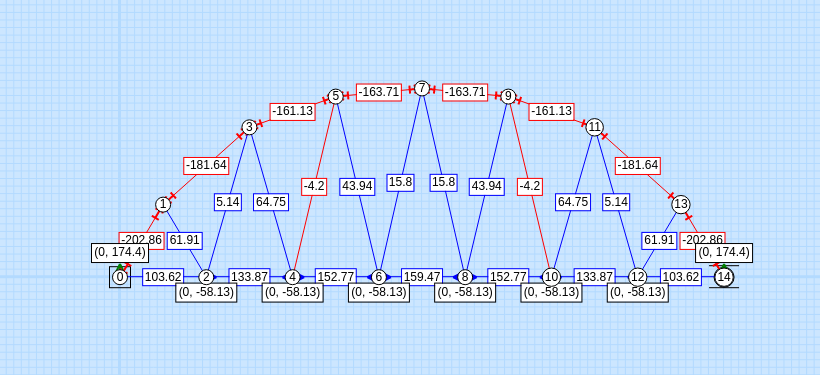
\includegraphics [width=.8\linewidth]{jhu}
	\caption{JHU simulation of bridge from generation code}
	\label{fig:jhu}
\end{figure}

The member list as desired has been provided in Figure \ref{fig:jhu-ml} as a table. All data is preserved.

\begin{figure}[H]
	\centering
	\begin{tabular}{|c|c|c|c|}
		\hline
		Number & Nodes & Length [cm] & Force [N] \\
		\hline
		0      & 0-2   & 11.43       & 103.6237  \\
		1      & 1-3   & 15.346      & -181.6391 \\
		2      & 2-4   & 11.43       & 133.8677  \\
		3      & 3-5   & 12.133      & -161.132  \\
		4      & 4-6   & 11.43       & 152.7701  \\
		5      & 5-7   & 11.481      & -163.7148 \\
		6      & 6-8   & 11.42       & 159.4714  \\
		7      & 7-9   & 11.481      & -163.7148 \\
		8      & 8-10  & 11.43       & 152.7701  \\
		9      & 9-11  & 12.133      & -161.132  \\
		10     & 10-12 & 11.43       & 133.8677  \\
		11     & 11-13 & 15.346      & -181.6391 \\
		12     & 12-14 & 11.43       & 103.6237  \\
		13     & 0-1   & 11.178      & -202.8626 \\
		14     & 1-2   & 11.183      & 61.9078   \\
		15     & 2-3   & 20.655      & 5.136     \\
		16     & 3-4   & 20.658      & 64.7467   \\
		17     & 4-5   & 24.592      & -4.1965   \\
		18     & 5-6   & 24.594      & 43.9376   \\
		19     & 6-7   & 25.644      & 15.7971   \\
		20     & 7-8   & 25.644      & 15.7971   \\
		21     & 8-9   & 24.594      & 43.9376   \\
		22     & 9-10  & 24.592      & -4.1965   \\
		23     & 10-11 & 20.658      & 64.7467   \\
		24     & 11-12 & 20.655      & 5.136     \\
		25     & 12-13 & 11.183      & 61.9078   \\
		26     & 13-14 & 11.178      & -202.8626 \\
		\hline
	\end{tabular}
	\caption{Member list from JHU}
	\label{fig:jhu-ml}
\end{figure}

\section{Task 6}

\label{sec:f-calc}

% Koden for utførelse av task 6 er lokalisert i Appendix \ref{sec:jhu-gen} sammen med JHU-gen koden. Kjører du programmet så ser du at den printer all informasjon som skal til. Dette er \lstinline{total_force_irl} og \lstinline{pascal} som svar på 6a, \lstinline{roind(distribution,2)} er svar på 6b, \lstinline{total_force_model} og \lstinline{round(total_force_model/g,2)} er svar på 6c.

\begin{figure}[H]
	\centering
	\begin{subfigure}{.8\linewidth}
		\centering
		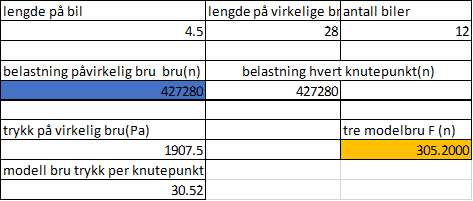
\includegraphics [width=.8\linewidth]{task-6-abc}

		\caption{Task 6 ABC numeric}
		\label{fig:6abc:num}
	\end{subfigure}
	\begin{subfigure}{.8\linewidth}
		\centering
		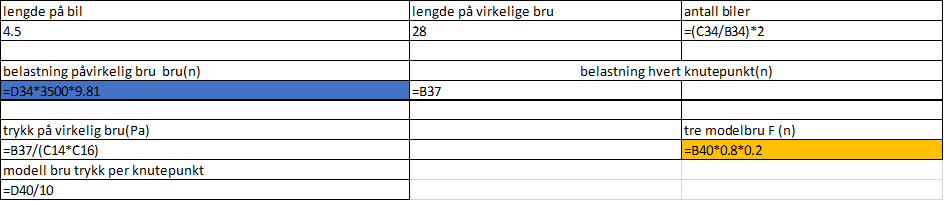
\includegraphics [width=.8\linewidth]{task-6-abc-formulas}

		\caption{Task 6 ABC formulas}
		\label{fig:6abc:form}
	\end{subfigure}
	\caption{Task 6 ABC}
	\label{fig:6abc}
\end{figure}

\subsection{D}

In the attached Figure \ref{fig:6d} we have all of the details for evaluation of member forces. Note the forces of the model and the sim are the same. This stems from the python program specified in Appendix \ref{sec:jhu-gen} generating an accurate representation of the bridge.

\begin{figure}[H]
	\centering
	\begin{subfigure}{.8\linewidth}
		\centering
		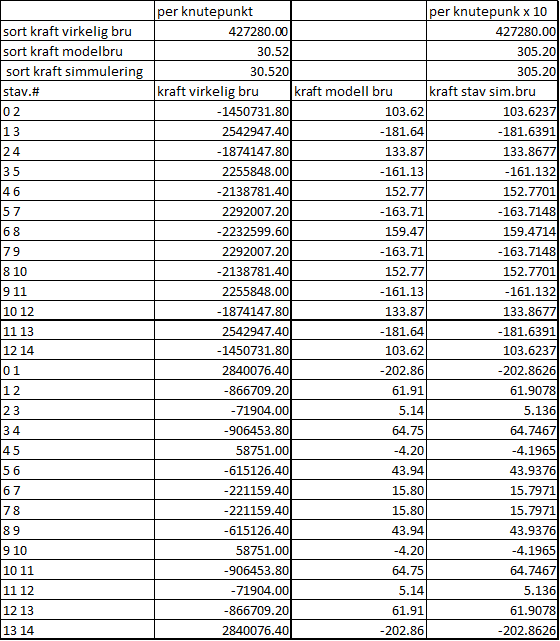
\includegraphics [width=.8\linewidth]{task-6D}

		\caption{Task 6D numeric}
		\label{fig:6d:num}
	\end{subfigure}
	\begin{subfigure}{.8\linewidth}
		\centering
		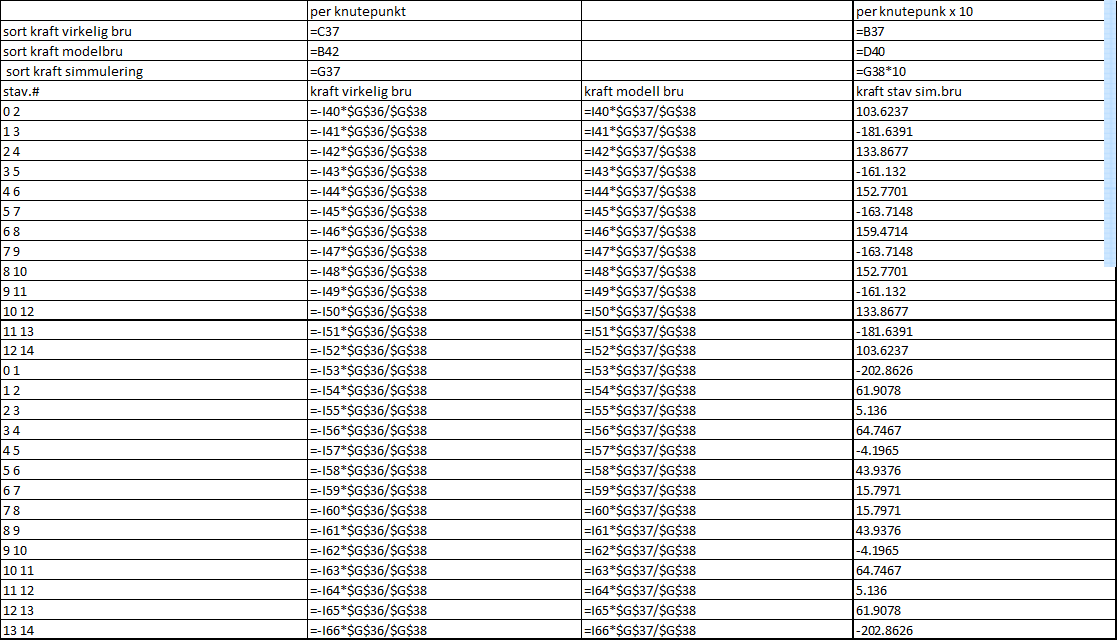
\includegraphics [width=.8\linewidth]{task-6D-formulas}

		\caption{Task 6D formulas}
		\label{fig:6d:form}
	\end{subfigure}
	\caption{Task 6D}
	\label{fig:6d}
\end{figure}

\section{Task 7}

\subsection {Why $\cosh$}

We decided to model the bridge after a $\cosh$ curve. This was based on that a catenary curve is the curve that minimizes potential energy of a function \cite{wiki:catenery}. Through this property it is also the strongest possible curve with a given length. Meaning theoretically we would get the strongest possible arch of a bridge mathematically possible.

\subsection {Errors during construction}

During our first iteration of the bridge we used spherical nodes. This was detrimental for multiple reasons

\begin{enumerate}
	\item It wastes plastic; we do not need horizontal roll tolerance, this would be the only contribution.
	\item Its hard to print; we need large quantities of supports and in some situations the supports that were added could not be removed
\end{enumerate}

\subsection {Features of the final bridge}

\subsubsection {Percentage extending base-beams}

Through the design we noticed we required a more powerful connection between the baselines nodes and its beams. To counteract this we decided to extend the base-nodes with a factor of \lstinline{BASE_RESIZE = 6}. This can be seen used at Appendix \ref{sec:openscad}:\ref{line:brescale}.

\subsubsection {Stabilizing back-plate}

Through testing we noticed how extending the rods would make then unstable and allow them to snap. T avoid this we decided to construct a polygonal back-plate for these rods. This can be found in Appendix \ref{sec:openscad}:\ref{line:backplate}. The programming pattern used was static single-assignment form \cite{wiki:ssaf}.

\subsubsection {Internalized standoff}

During construction of the bridge we had to sand down the beams to be able to mount them together. This made construction of the bridge notably harder. To combat this we added internalized standoffs. These were placed there so beams could be directly inserted into the rods without needing any extra sanding. This added quite a bit of complexion to the code and the actual typoral location of where this occurred can not be found.

\subsubsection {Node indexing}

Following our first print batch we noticed we had a small issue; we could not identify the correct nodes (note at this point our nodes were spherical). To combat this we added indexes to each point. Confusingly the indexes on the model (SCAD space) are separate from in JHU (JHU space). This stems from the JHU code being made as simple as possible while the SCAD code quite a bit more complicated.

\subsubsection {Cross section margin connections}

We noticed how crossing member were poorly connected to the other side through the fact that the rod had little material. To fix this we added a margin designed to cross the gap between them.

\subsubsection {Lamination direction}

We decided that the lamination direction of the print would have a large impact on the structural integrity of the nodes. To deal with this we printed in the direction the forces would perpetrate through the nodes.

\section{Task 8}
\label{sec:8}

During testing we progressively increased the force we applied to the bridge. We hit our threshold of $35\mathrm{kg}$ found in Section \ref{sec:f-calc}. After we hit this threshold out of pure spite we decided to continue until the bridge snapped. This stems from long painful work and low sentimental commitment. We finally reached $80\mathrm{kg}$. During this we would expect the arch to snap first (stemming from Figure \ref{fig:jhu}). This was not what we saw. We noted the snap was the member between the nodes 6 and 7 in SCAD space. This deformation can be seen in progress in Figure \ref{fig:deform}. We are unsure what caused this. Our strongest hypothesis is that there was a lacking quantity of glue in the 6th node. This arises from inspecting that that Node 7 contained wood remains. This can be seen in Figure \ref{fig:snap:7}. As opposed to this we can see that the joint in node 6 did not contain this potentially signalling that the beam simply slid out when the force got too great. This can be seen in Figure \ref{fig:snap:6}.

\begin{figure}[H]
	\centering
	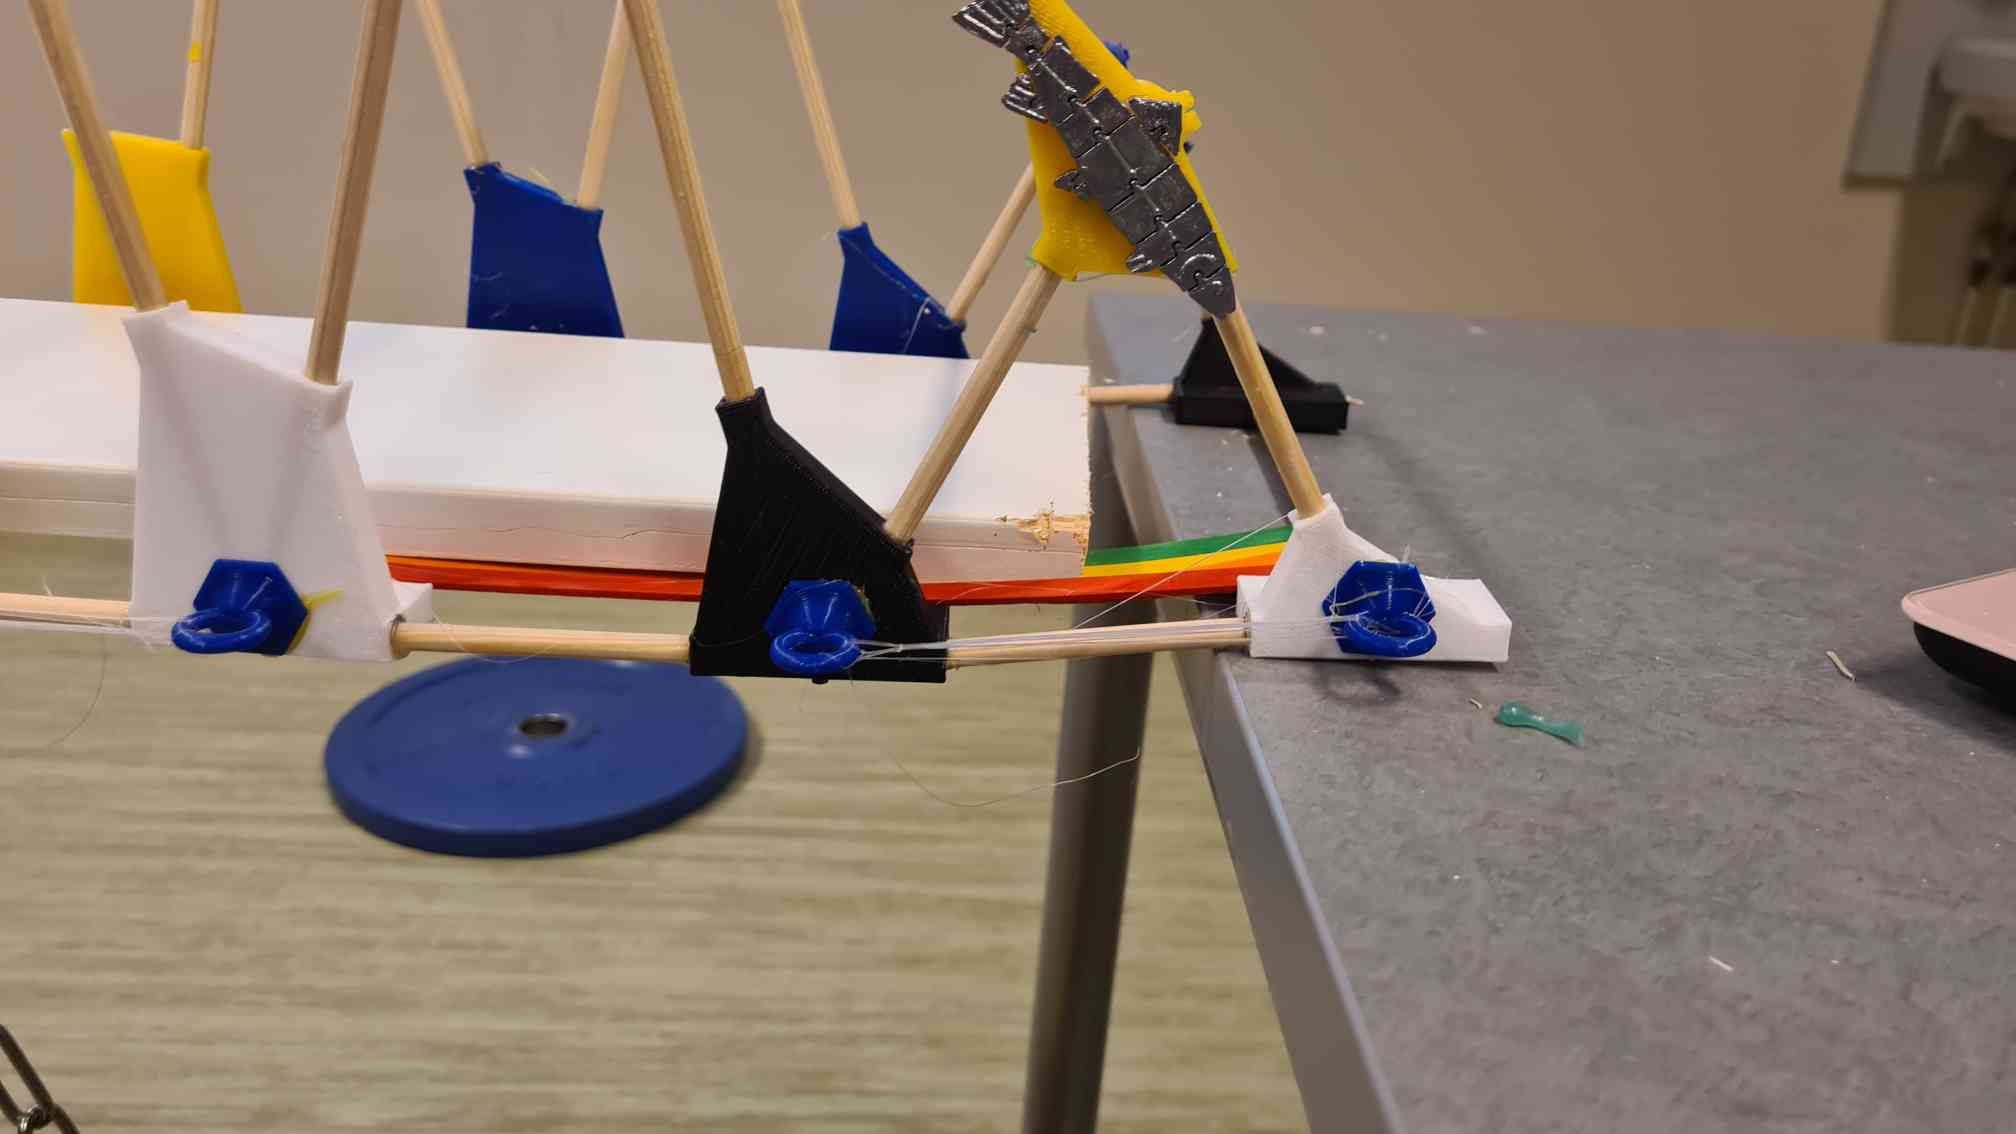
\includegraphics [width=.8\linewidth]{bend-closer}
	\caption{Deformation of nodes 6 \and 7}
	\label{fig:deform}
\end{figure}

\begin{figure}[H]
	\begin{subfigure}{.5\textwidth}
		\centering
		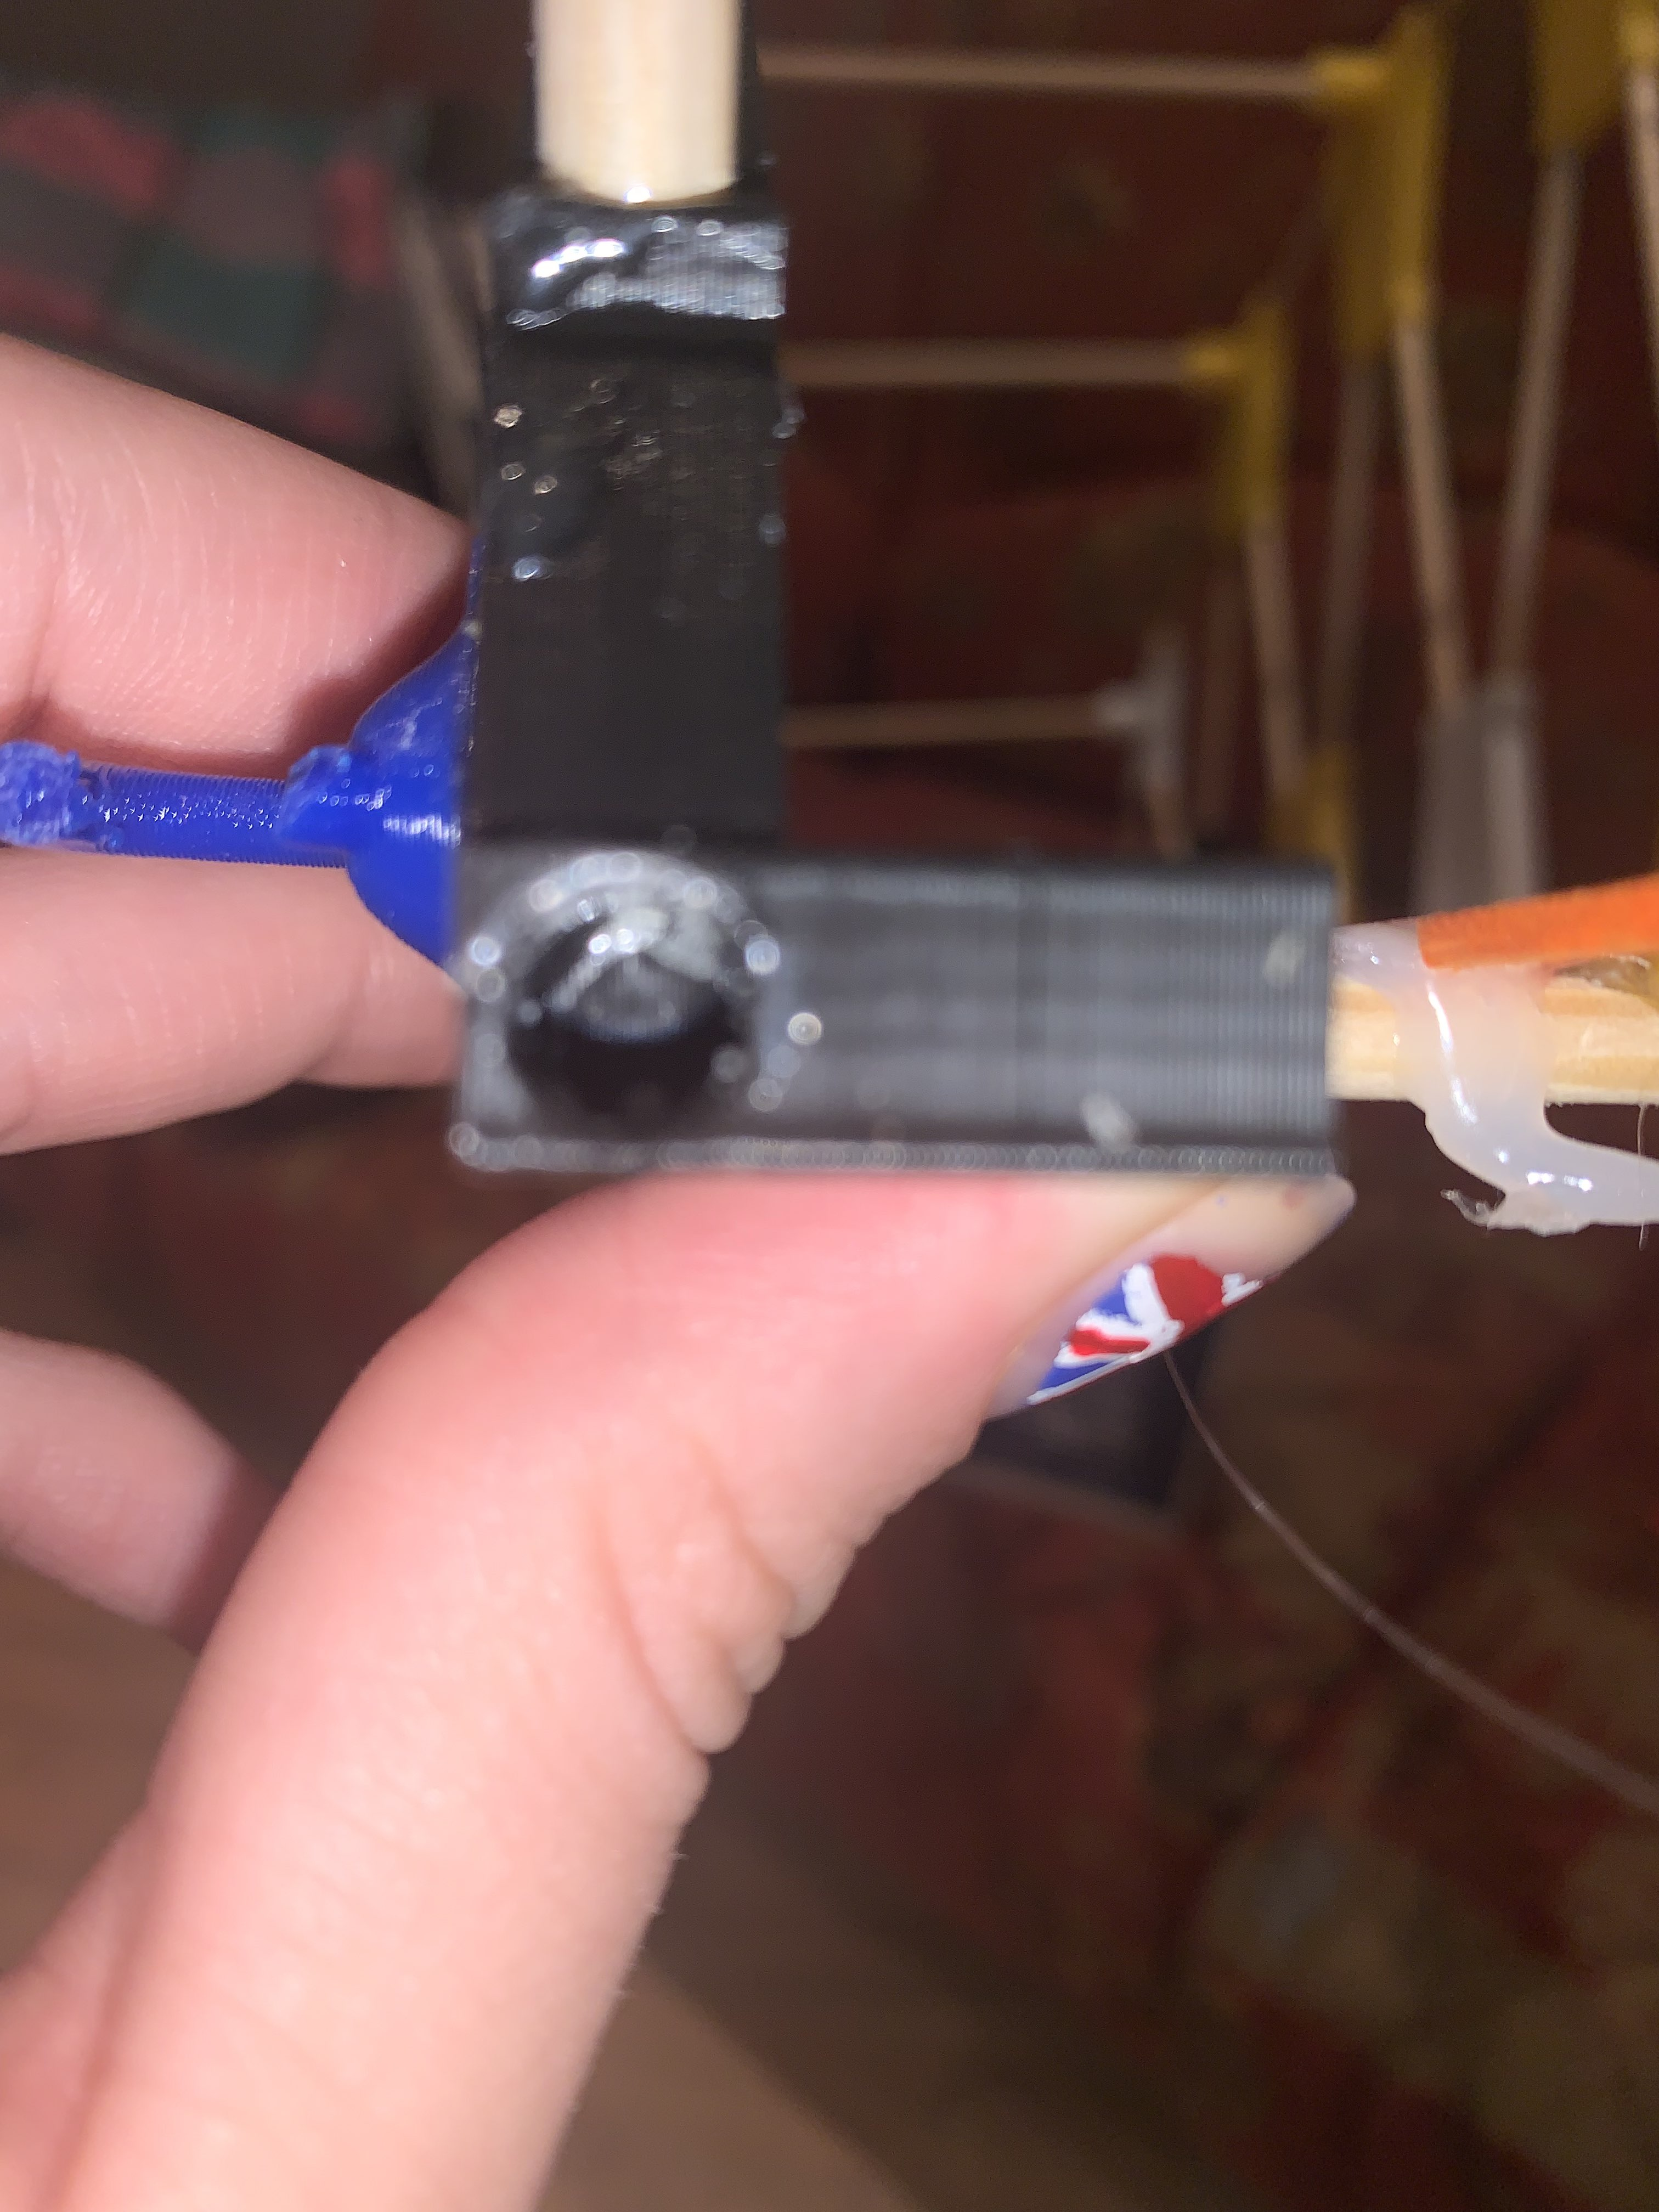
\includegraphics[width=\subimgw,trim={0 40cm 0 5cm},clip]{beam-6}

		\caption{node 7 snap joint}
		\label{fig:snap:7}
	\end{subfigure}%
	\begin{subfigure}{.5\textwidth}
		\centering
		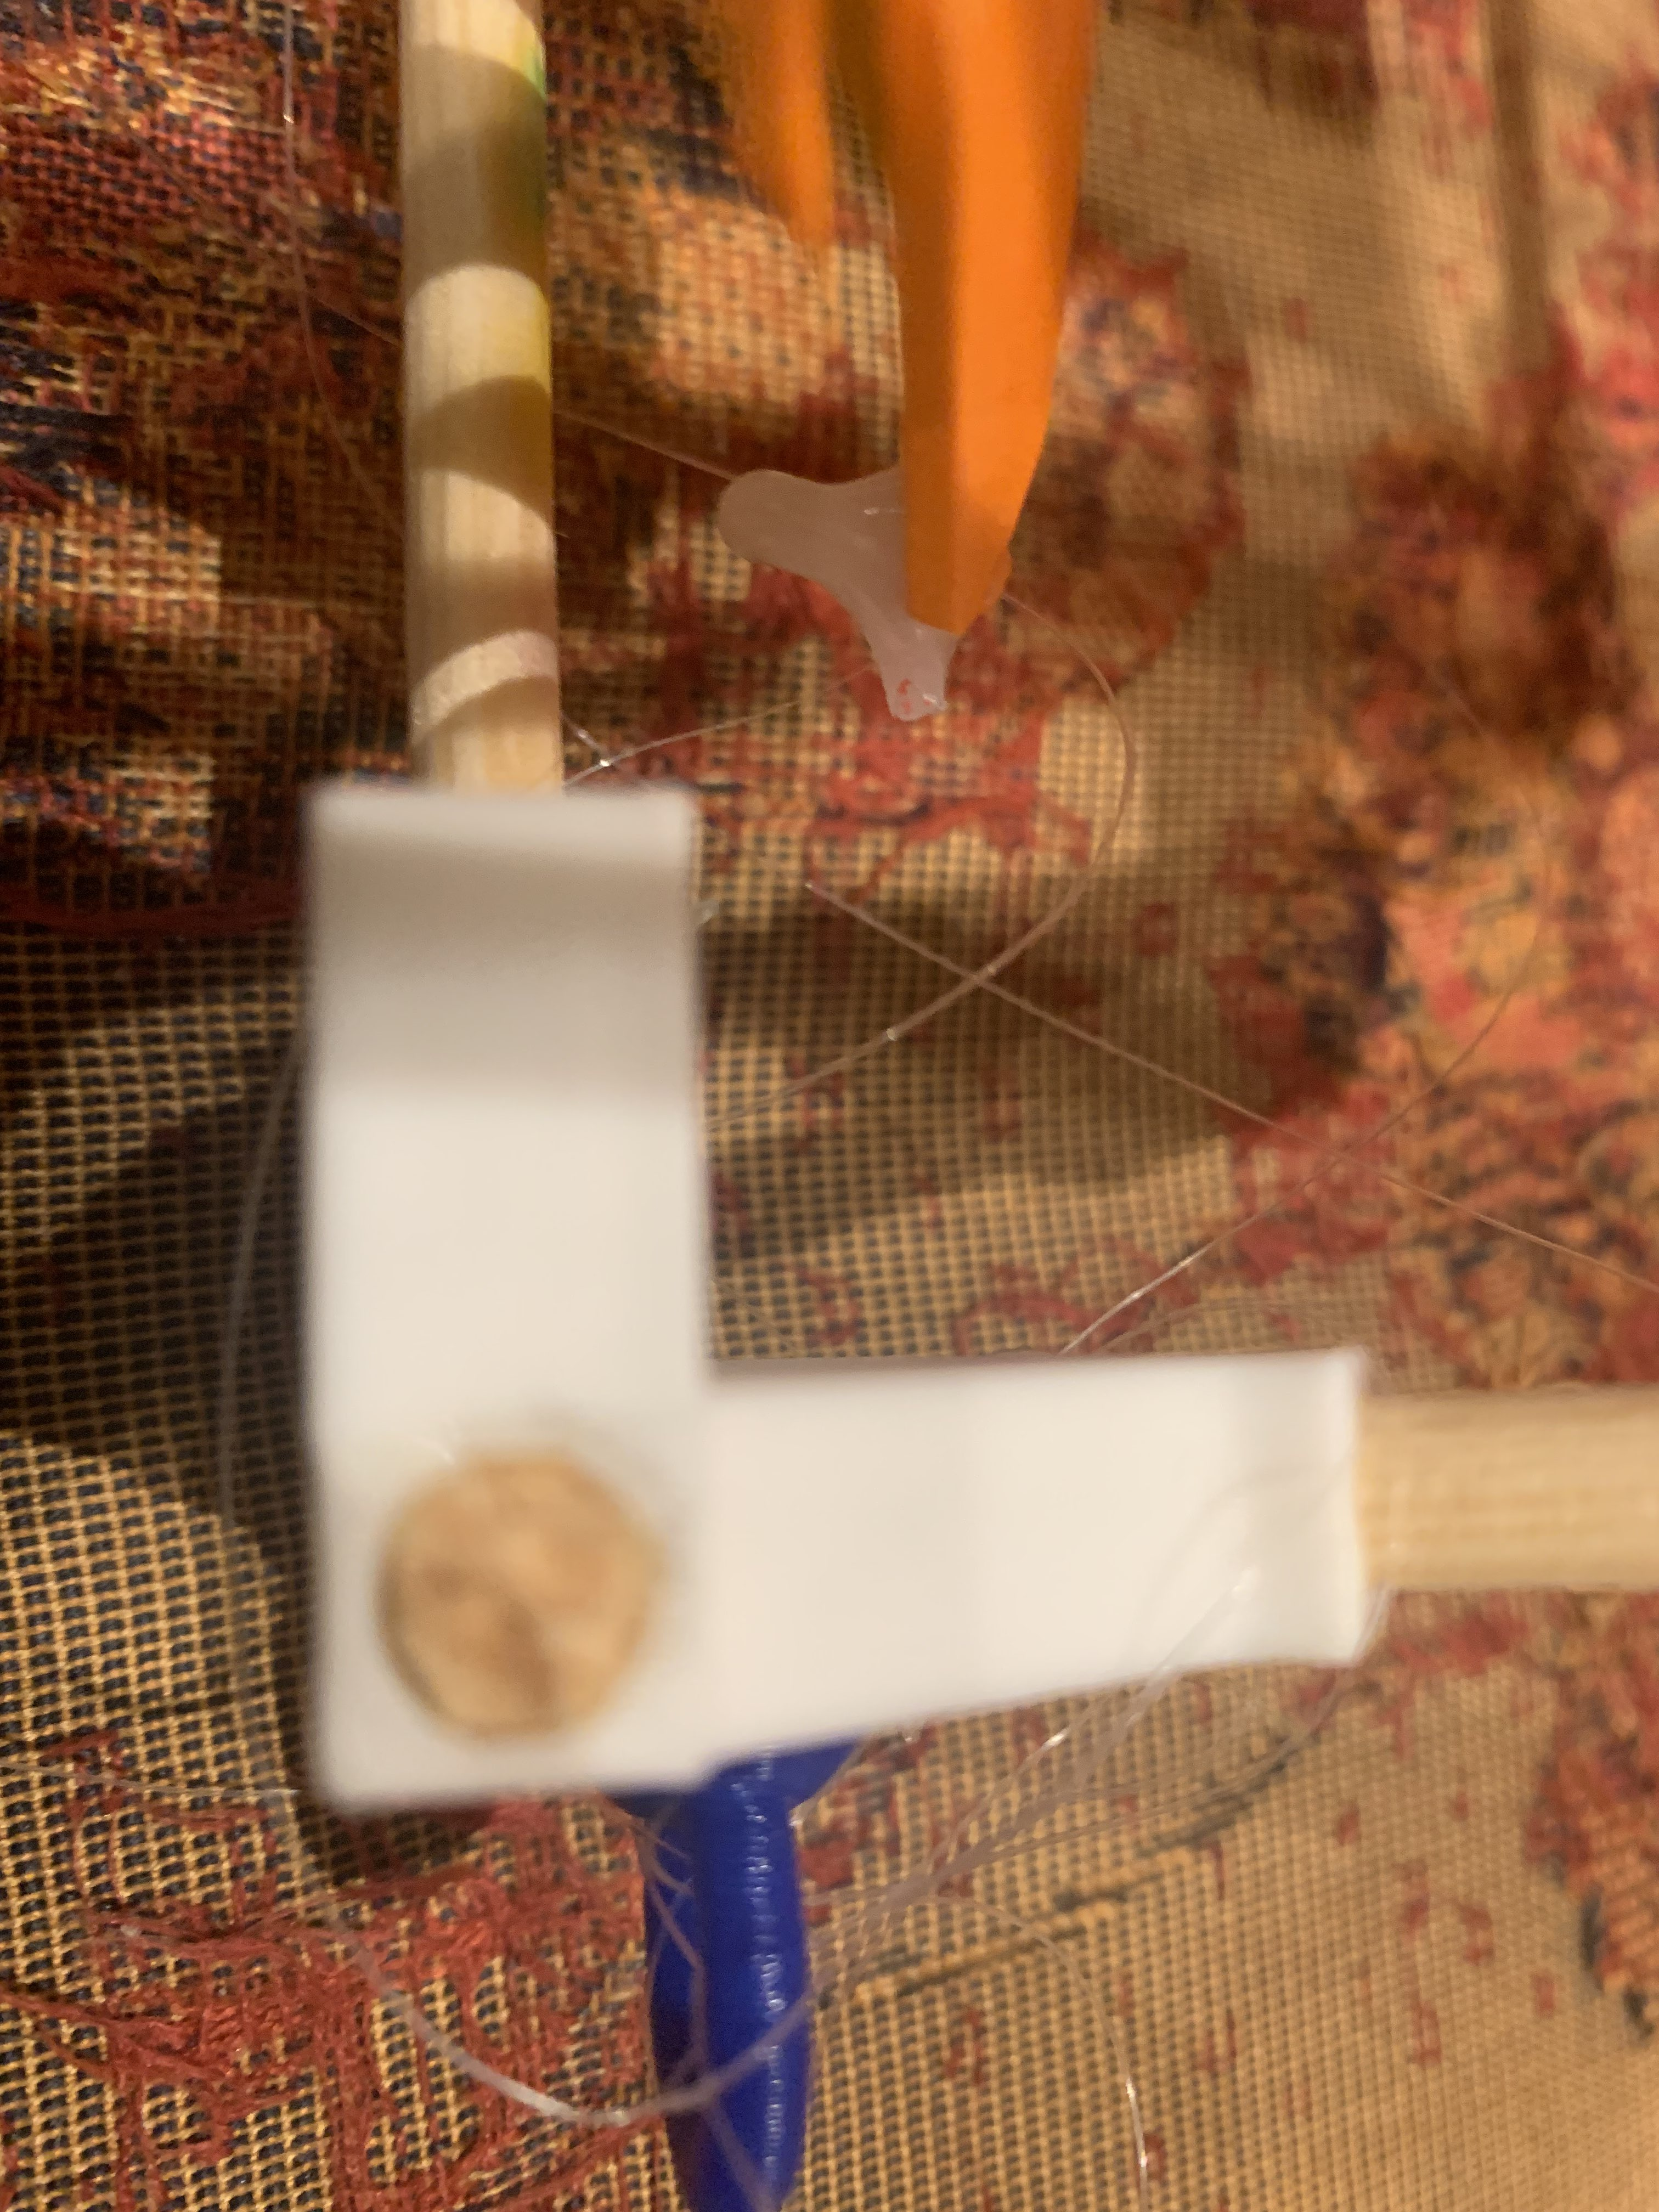
\includegraphics[width=\subimgw,trim={0 5cm 0 40cm},clip]{beam-7}

		\caption{node 6 snap joint}
		\label{fig:snap:6}
	\end{subfigure}

	\caption{nodes between the broken member}
	\label{fig:snap}
\end{figure}

\section{Task 9}

\subsection{a}

After constructing the basis for the bridge out of solely biodegradable and recyclable materials \cite{wiki:pla}. This aligns with our ideas of a ecological and green solution for the bridge.

On top of this we have added a solar panel as decoration of the bridge. This is to represent how in the final version solar panels will be prevalent through the construction.

Other decorations include theming the bridge around pride and accidentally making Rainbow Road from Mario Kart. See Figure \ref{fig:gey} for a visual comparison.

Finally we decorated the bridge with Lofoten themed decore such as Fish and Fishing equipment.

\begin{figure}[H]
	\begin{subfigure}{.5\textwidth}
		\centering
		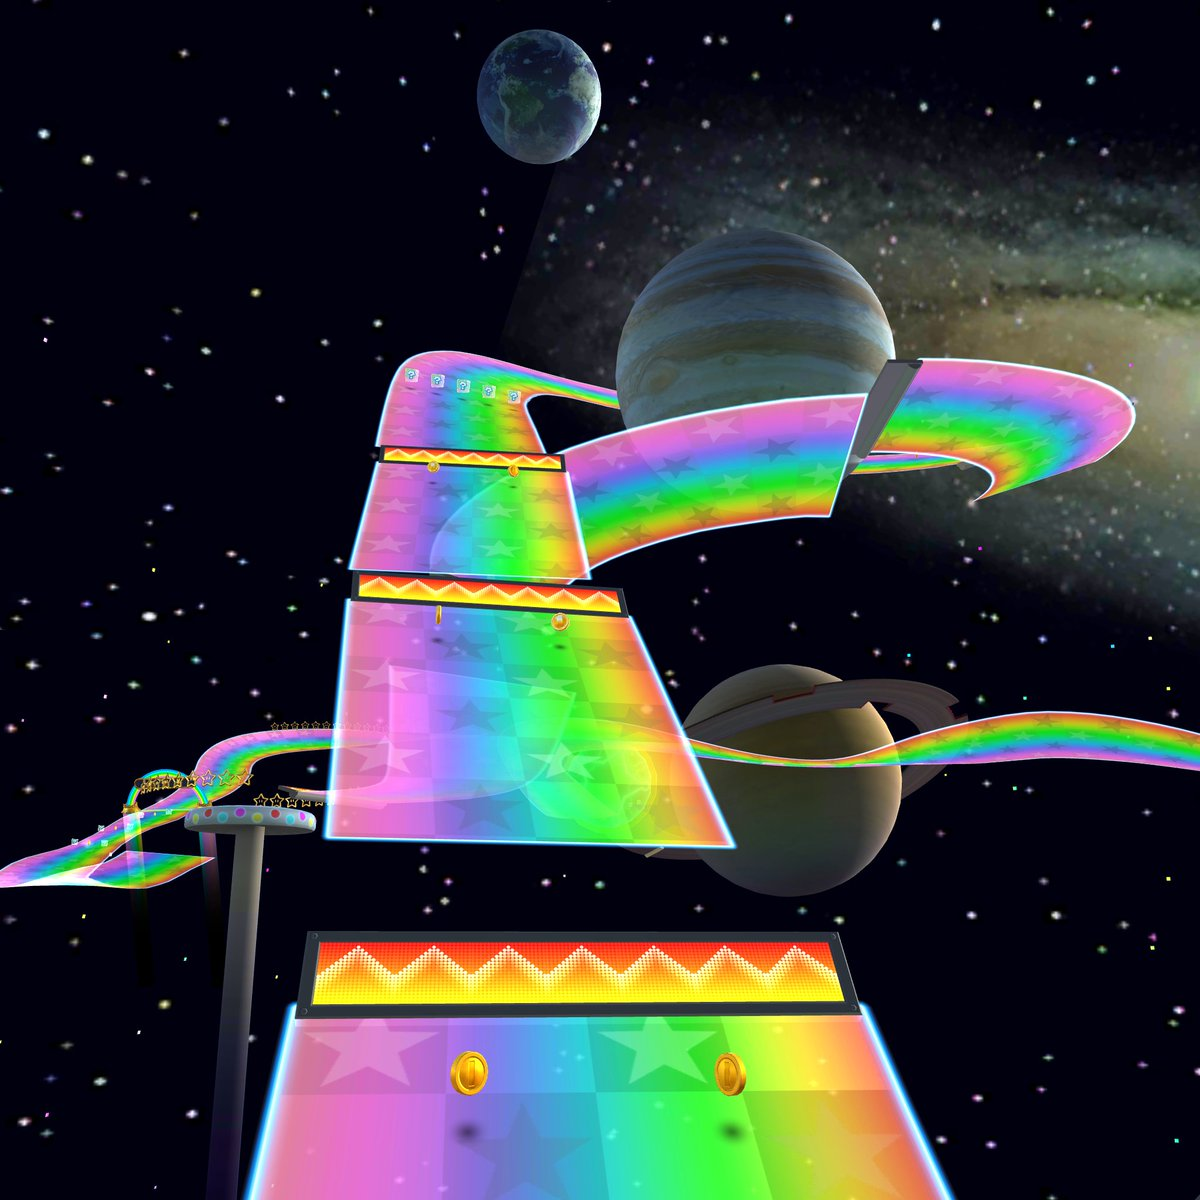
\includegraphics[width=\subimgw,trim={0 10cm 0 0},clip]{rainbow-road}

		\caption{Rainbow Road}
	\end{subfigure}%
	\begin{subfigure}{.5\textwidth}
		\centering
		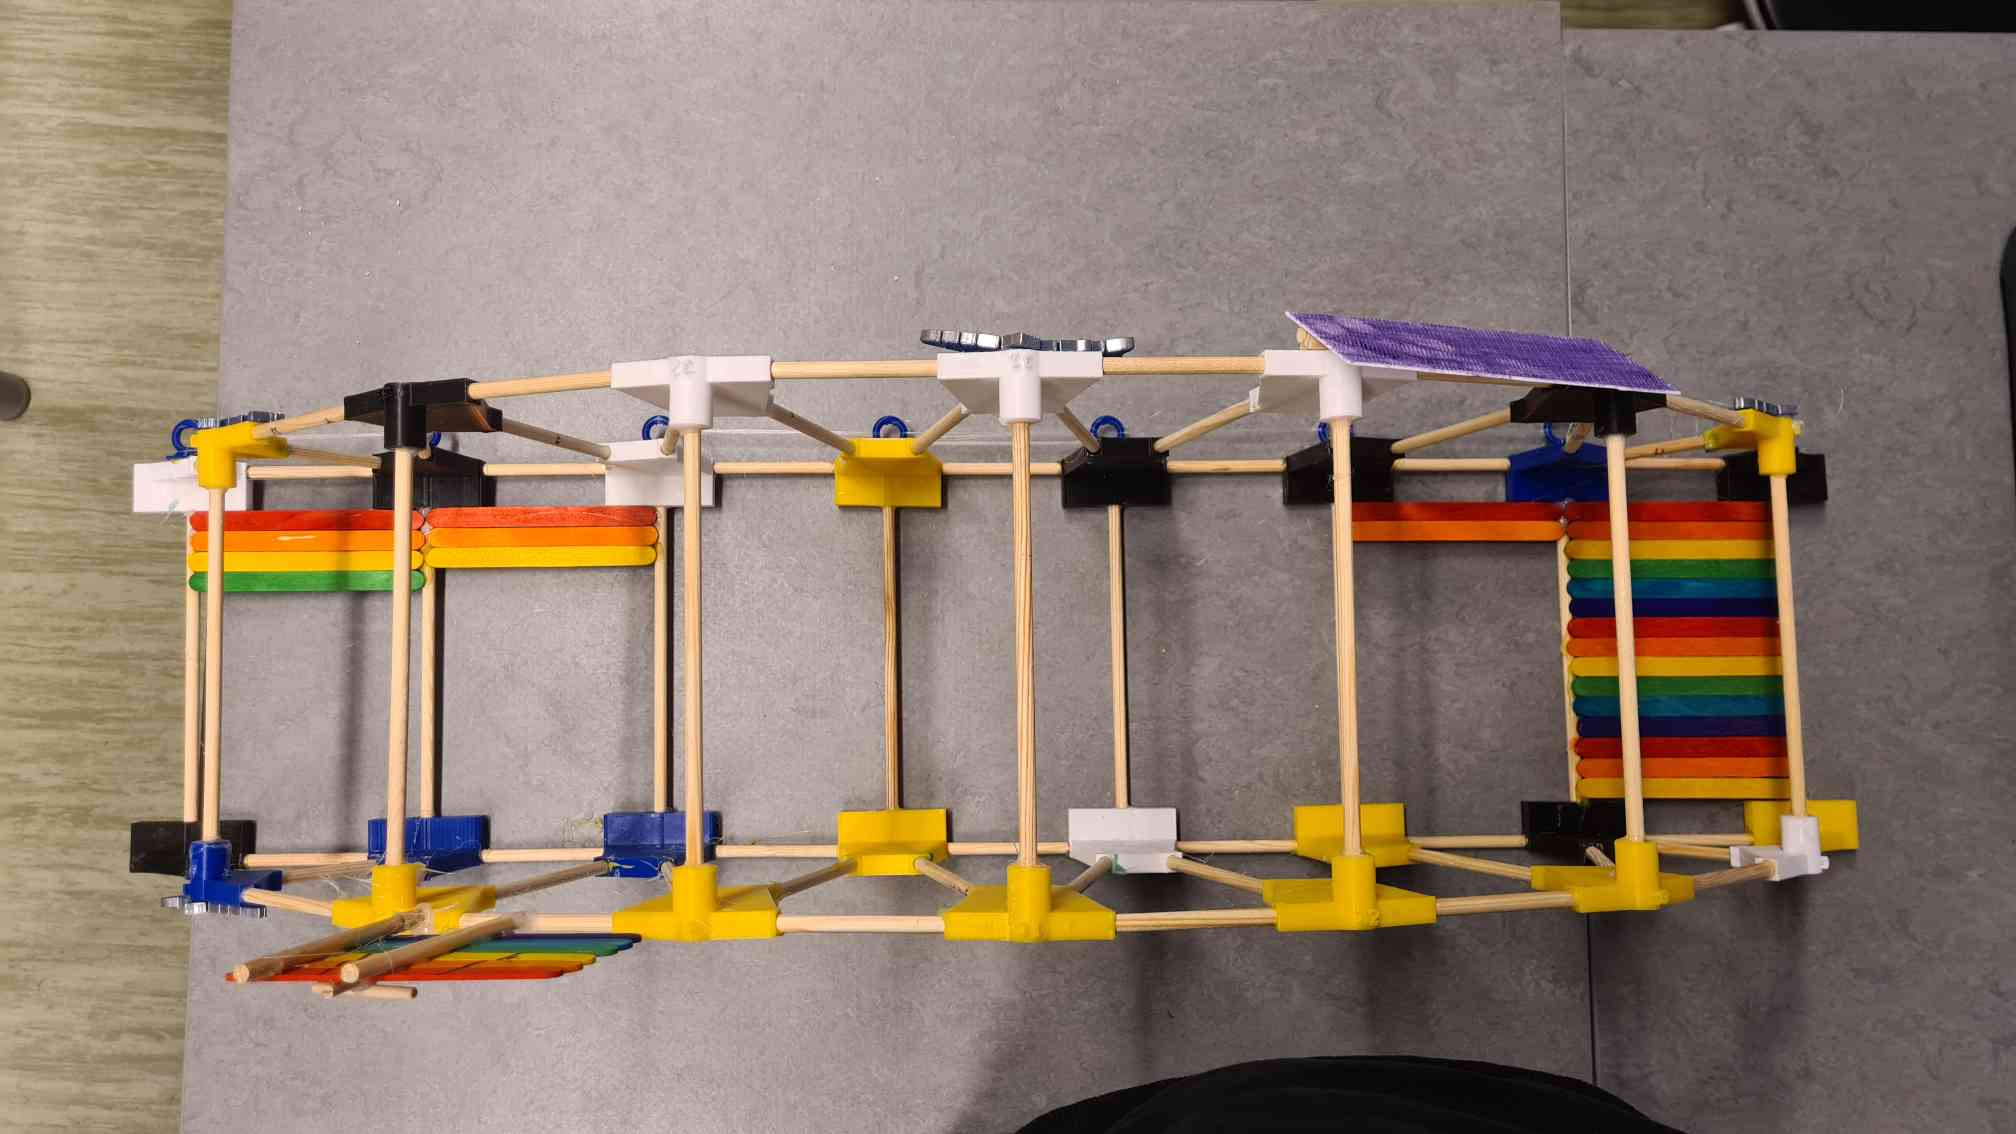
\includegraphics[width=\subimgw,trim={0 0 0 0},clip]{top}

		\caption{Bridge top-view}
	\end{subfigure}

	\caption{Comparison of bridge and rainbow road}
	\label{fig:gey}
\end{figure}

\subsection{b}

\subsection{c}

During testing of the bridge we noticed the load being placed on the baseline of the bridge was larger than expected both through intuition and following the simulations found in Figure \ref{fig:jhu}. This has lead us to desire to modify the joint generation code to include variable radius beams. This feature would require quite a bit more code and manual labour. Through avoiding this we have constructed the strongest tested bridge that does not employ thicker beams.

\chapter{Appendix}

\section{Reference to OpenSCAD code}
\label{sec:openscad}

\lstinputlisting[escapechar=~]{../bridge.scad}

\section{Recrence to Python JHU-generation code}
\label{sec:jhu-gen}

\lstinputlisting[language=Python]{../jhu-gen.py}

\addcontentsline{toc}{section}{List of figures}
\listoffigures

\bibliography{report}

\end{document}
